\documentclass[t,compress,mathserif,12pt,xcolor=dvipsnames]{beamer}
\setbeamertemplate{bibliography item}{\insertbiblabel}
\usepackage{etex}
\reserveinserts{28}
\definecolor{bleuUni}{RGB}{0, 157, 224}
\definecolor{marronUni}{RGB}{68, 58, 49}
\usecolortheme[named=bleuUni]{structure}
\usepackage[bars]{beamerthemetree} % Beamer theme v 2.2
\usepackage{multimedia}
\usepackage[utf8]{inputenc}
%\usepackage[frenchb]{babel}
\usepackage[T1]{fontenc}
\usepackage{kmath,kerkis}
\usepackage{xmpmulti}
%\usepackage{mathpazo}
%\usepackage[bitstream-charter]{mathdesign}
%\usepackage{lmodern}
\usepackage{booktabs}
\usepackage{multirow}
\usepackage{pgfplots}
\pgfplotsset{compat=newest}
\usepackage{tikz}
\usetikzlibrary{patterns, shapes, arrows}
\usepackage{mathtools}
\usepackage{listings}
\usepackage{eulervm}
\usepackage{pifont}% http://ctan.org/pkg/pifont
\newcommand{\cmark}{\ding{51}}%
\newcommand{\xmark}{\ding{55}}%
\lstset{
  language=C++,
  basicstyle=\tiny\ttfamily,
  numbers=left,
  numberstyle=\tiny\ttfamily,
  stepnumber=1,
  numbersep=5pt,
  backgroundcolor=\color{white},
  showspaces=false,
  showstringspaces=false,
  showtabs=false,
  frame=single,
  tabsize=2,
  captionpos=b,
  breaklines=true,
  breakatwhitespace=false,
  escapeinside={(*@}{@*)},
  identifierstyle=\ttfamily,
  keywordstyle=\color[rgb]{0,0,1},
  commentstyle=\color[rgb]{0.133,0.545,0.133},
  stringstyle=\color[rgb]{0.627,0.126,0.941},
  moredelim=[is][\underbar]{**}{**},
}

\lstdefinestyle{mycpp}
{
    language = C++,
    % numbers=left,
    % numbersep=0.3em,
    escapeinside={(*@}{@*)},
    tabsize=2,
    % basicstyle=\tiny\ttfamily,
    morekeywords = {constexpr,int8_t,int16_t,int32_t, size_t},
    % commentstyle=\color{comment-color},
}

\usepackage[backend=biber, style=ieee]{biblatex}
\addbibresource{bibli.bib}
\renewcommand\mkbibacro[1]{{\footnotesize\MakeUppercase{#1}}}

\mode<presentation>
\newcommand*\oldmacro{}%
\let\oldmacro\insertshorttitle%
\renewcommand*\insertshorttitle{%
 \oldmacro\hfill%
\insertframenumber\,/\,\inserttotalframenumber}
\setbeamertemplate{footline}[frame number]
\setbeamersize{text margin left=10pt,text margin right=10pt}
\setbeamerfont{frametitle}{size=\large}
\setbeamertemplate{frametitle}{ \nointerlineskip \begin{beamercolorbox}[wd=\paperwidth,ht=2.2ex,dp=0.5ex,left]{frametitle} \hspace*{3.1ex}\strut\bfseries\color{bleuUni!15!white}\insertframetitle\strut\par \end{beamercolorbox}}

\setbeamertemplate{bibliography item}{\insertbiblabel}


\makeatletter
\def\beamer@andinst{\\[0.1em]}
\makeatother
%~~~~~~~~~~~~~~~~~~~~~~~~~~~~~~~~~~~~~~~~~~~~~~~~~~~~~~~~~~~
%\setbeamercovered{higly dynamic}
\usetheme{Ilmenau} % Beamer theme v 3.0
%\useoutertheme[subsection=true]{smoothbars}%Beamer Outer Theme-circles on top
\setbeamercolor{section in head/foot}{bg=marronUni}

\useinnertheme{circles} %rectangle bullet points instead of circle ones
\usepackage{beamerthemebars}
\setbeamercolor{navigation symbols dimmed}{fg=red!80!black}
\setbeamercolor{navigation symbols}{fg=red!80!black}
\setbeamertemplate{navigation symbols}{}%remove navigation symbols
%~~~~~~~~~~~~~~~~~~~~~~~~~~~~~~~~~~~~~~~~~~~~~~~~~~~~~~~~~~~~~~~~~~~~~
\title{\textbf{Décodage de codes polaires sur des architectures programmables}}
%\subtitle{algorithms et arhitecture}\hspace{10.7cm}
\author[Mathieu Léonardon\hspace{7.51cm}{mathieu.leonardon@ims-bordeaux.fr}]    {Mathieu Léonardon}
\titlegraphic{
\includegraphics[height=1cm]{logos/ims.png} \hfil %
              
\includegraphics[height=1cm]{logos/inp.PNG} \hfil %
              
\includegraphics[height=1cm]{logos/ub.png}  \hfil %
              
\includegraphics[height=1cm]{logos/poly.eps}}
\date{13 Décembre 2018}
%\pgfdeclareimage[height=.8cm]{logo_ISCAS}{index.png}
%\logo{\pgfuseimage{logo_ISCAS}\hspace{\dimexpr\paperwidth-3.55cm}\vspace{-8pt}}

\definecolor{dgreen}{rgb}{0.,0.6,0.}
\definecolor{milano}{rgb}{0.458824, 0.050980, 0.058824}
\definecolor{bahama}{rgb}{0.066667, 0.298039, 0.443137}
\definecolor{blupres}{RGB}{0, 157, 224}
\definecolor{redpres}{RGB}{204, 0, 0}

\newcommand\blfootnote[1]{%
  \begingroup
  \renewcommand\thefootnote{}\footnote{#1}%
  \addtocounter{footnote}{-1}%
  \endgroup
}

\newcommand{\RED} [1]{\textcolor{red}{\textbf{#1}}}
\newcommand{\ORANGE} [1]{\textcolor{orange}{\textbf{#1}}}
\newcommand{\GREEN} [1]{\textcolor{dgreen}{\textbf{#1}}}
\newcommand{\BLUE} [1]{\textcolor{blue}{\textbf{#1}}}

\newcommand{\MILANO} [1]{\textcolor{milano}{#1}}
\newcommand{\BAHAMA} [1]{\textcolor{bahama}{#1}}

\usepackage{textpos}
%\usepackage{stmaryrd}
\usepackage{amsbsy}
\usepackage{makecell}
%\usepackage{fourier-orns}
% \usepackage{tikz}
% \usetikzlibrary{patterns, shapes, arrows, shapes.multipart}

\usepackage{etoolbox}
\AtBeginSection[]
{
	\ifnumcomp{\value{section}}{=}{1}{}{
\begin{frame}[c]{Plan}
\centering
\tableofcontents[
  currentsection,
  currentsubsection,
]
\end{frame}
}
}
\AtBeginSubsection[]
{
	\begin{frame}[c]{}
\tableofcontents[
currentsection,
sectionstyle=show/show,
subsectionstyle=show/shaded/hide
]
	\end{frame}
}


% \defbeamertemplate*{title page}{customized}[1][]
% {
%   \usebeamerfont{title}\inserttitle\par
%   \usebeamerfont{subtitle}\usebeamercolor[fg]{subtitle}\insertsubtitle\par
%   \bigskip
%   \usebeamerfont{author}\insertauthor\par
%   \usebeamerfont{institute}\insertinstitute\par
%   \usebeamerfont{date}\insertdate\par
%   \usebeamercolor[fg]{titlegraphic}\inserttitlegraphic
% }

\bibliography{bibli}

\begin{document}

\begin{frame}[c]
\titlepage
\end{frame}

\begin{frame}[c]
	\tableofcontents[
	subsectionstyle=hide,
	]
\end{frame}




\section[Introduction]{Introduction}
\subsection*{Les codes correcteurs d'erreurs}

\begin{frame}[c]
	\begin{center}
	\multiinclude[<+>][start=1,format=pdf,graphics={width=.8\textwidth}]{./fig/chaine_com}
	\end{center}
  	\frametitle<1>{Chaîne de communication}
  	\frametitle<2->{Chaîne de communication numérique}
	\begin{itemize}
		\item<1-> Message transmis au travers d'un canal de communication
		\item<2-> Nécessité d'une modulation
		\item<3-> Modèle simplifié
		\item<4-> Correction d'erreurs par ajout de redondance ($K>N$)
		\item<5-> Le cas des codes polaires
	\end{itemize}
\end{frame}

\begin{frame}
\vfill
	\begin{itemize}
		\item 1948 : Théorie de l’information (Shannon)
		\item 1950 : Codes de Hamming
		\item 1955 : Codes convolutifs
		\item 1960 : Codes BCH
		\item 1960 : Codes Reed-Solomon
		\item 1960 : Codes LDPC 
		\item 1966 : Codes concaténés (Forney)
		\item 1993 : \textbf{Codes turbos}
		\item 1996 : \textbf{LDPC rediscovery}
		\item 2008 : \textbf{Codes polaires}
	\end{itemize}
	\vfill
\end{frame}

\subsection*{Les codes polaires}
\begin{frame}[c]{Codage polaire}
	\begin{columns}[T] % align columns
		\begin{column}{.65\textwidth}
			\multiinclude[<+>][start=1,format=pdf,graphics={width=\textwidth}]{./fig/focus_polar}
		\end{column}
		\begin{column}{.35\textwidth}
		\begin{itemize}
			\item<1-> Graphe de factorisation
			\item<2-> Bits d'information
			\item<3-> Bits gelés
			\item<5-> Mot de code : $x_i$
		\end{itemize}
		\end{column}

	\end{columns}

\end{frame}
\subsection*{Le décodage SC}

\begin{frame}[c]{Algorithme de décodage SC}
	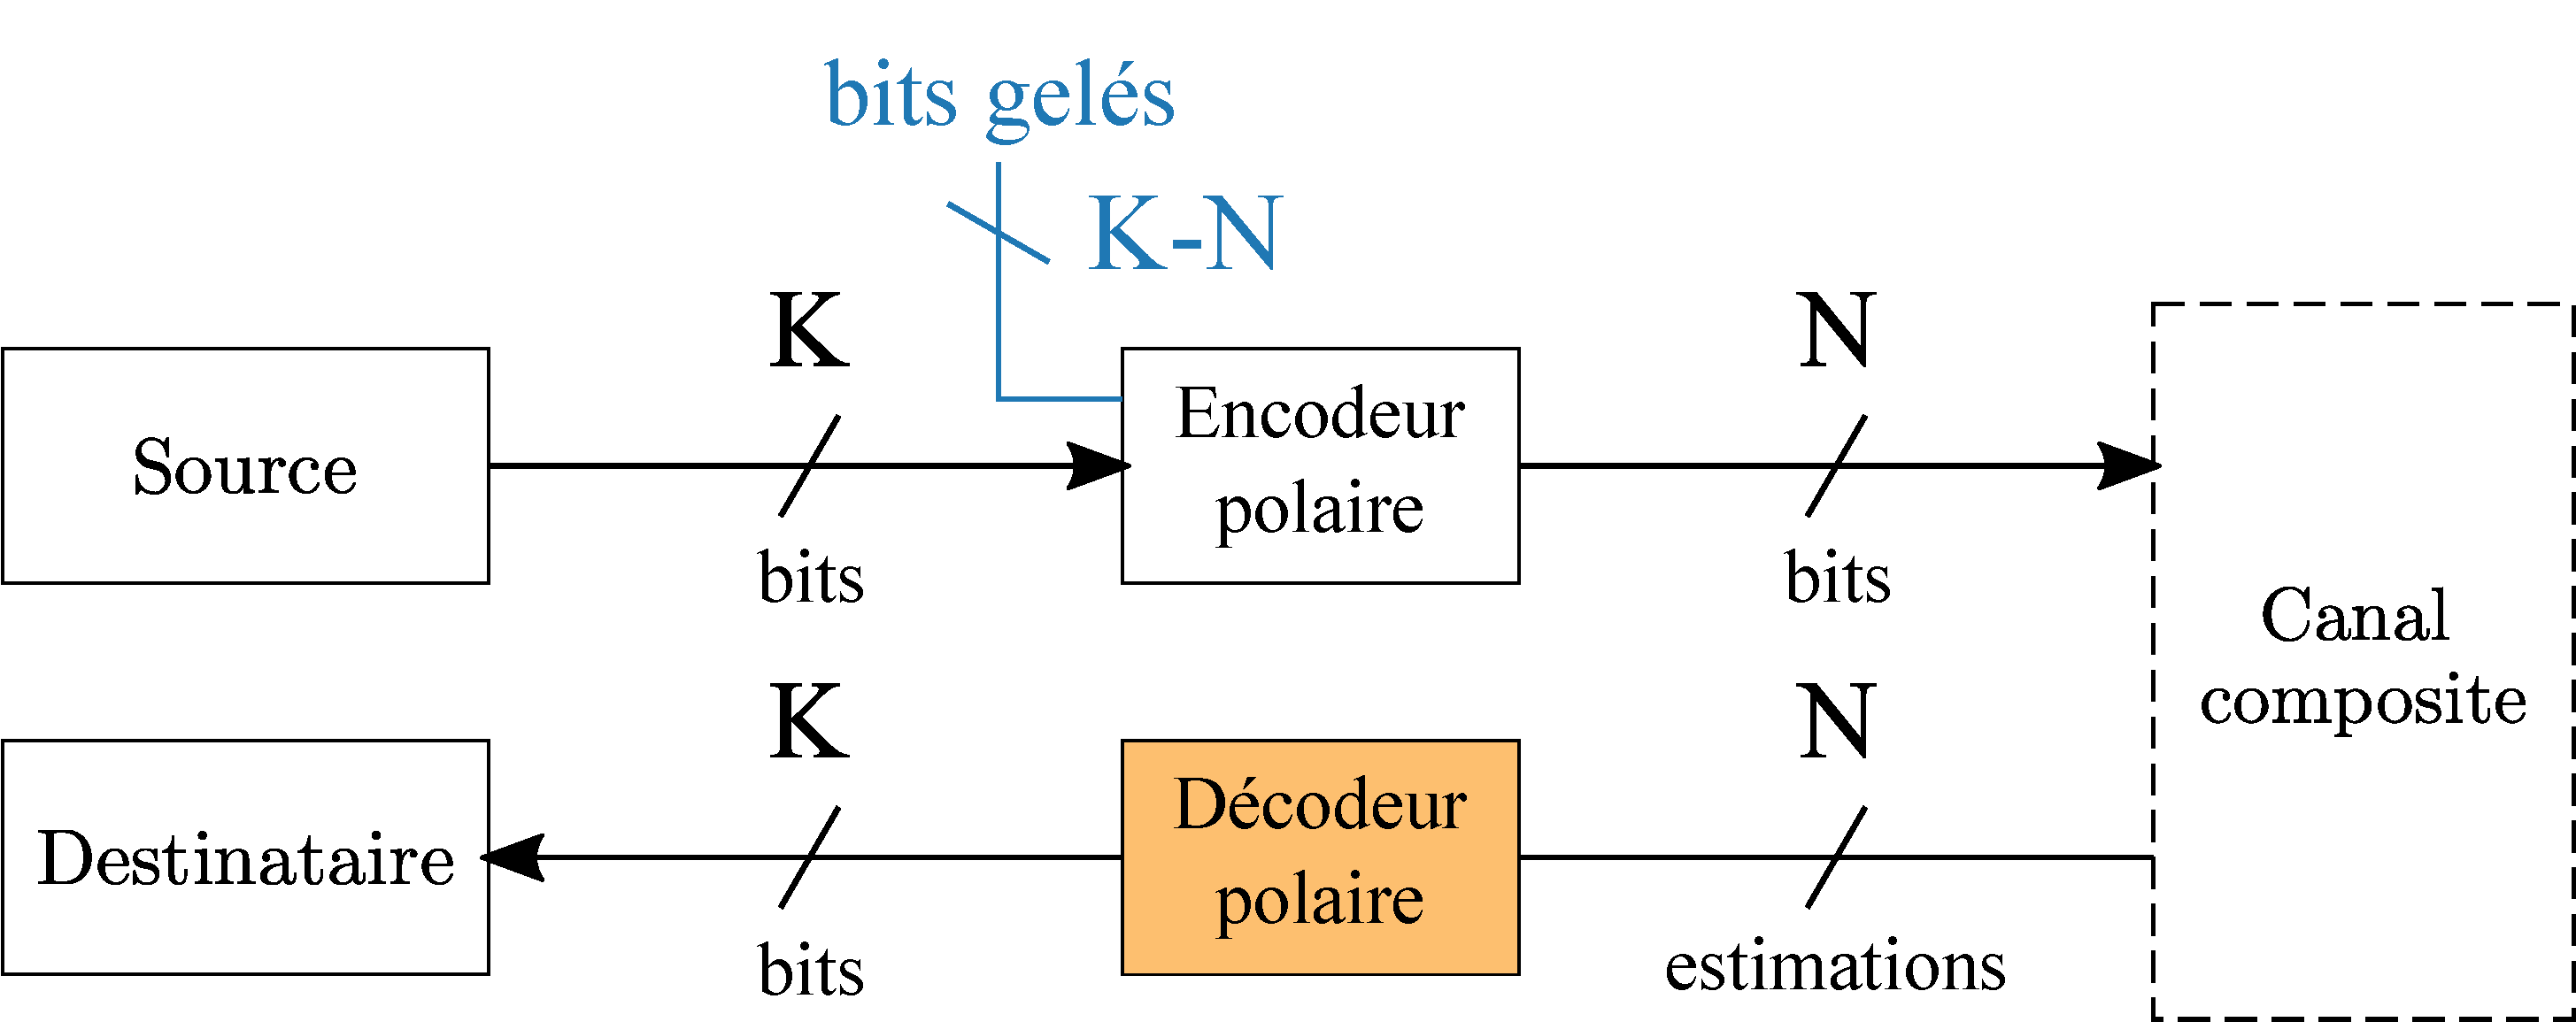
\includegraphics[width=.8\textwidth]{fig/decoder_in_chain.pdf}
\end{frame}

\begin{frame}[c]{Algorithme de décodage SC}
	\begin{columns}[T] % align columns
		\begin{column}{.65\textwidth}
			\multiinclude[<+>][start=1,end=2,format=pdf,graphics={width=\textwidth}]{./fig/focus_decoder}
		\end{column}
		\begin{column}{.35\textwidth}
		\begin{itemize}
			\item<1-> $L$ : Log Likelihood Ratios (LLR)
			\item<2-> Deux formats de données
		\end{itemize}
		\end{column}
	\end{columns}

\end{frame}

\begin{frame}[c]{Algorithme de décodage SC}
	\begin{columns}[T] % align columns
		\begin{column}{.35\textwidth}
			\multiinclude[<+>][start=1,format=pdf,graphics={width=\textwidth}]{./fig/polar_functions}    
		\end{column}

		\begin{column}{.65\textwidth}
		\only<1>{
		$$f(L_a,L_b) = \text{sign}(L_a.L_b).\min(|L_a|,|L_b|)$$
		\vspace{1.1cm}

		$$g(L_a,L_b,\hat{s}_a) = (1-2\hat{s}_a)L_a+L_b$$
		}

				\only<2>{
				\vspace{0.5cm}
		$$\texttt{R1}(L_a)  =  \left\{\begin{array}{l c l} 0 \text{ si } L_a \geq 0 \\ 1 \text{ si } L_a < 0 \end{array}\right.$$
		\vspace{1.1cm}

		$$h(\hat{s}_a,\hat{s}_b) = (\hat{s}_{a} \oplus \hat{s}_{b}, \hat{s}_{b})$$
		}
		\end{column}

	\end{columns}

	
 %    g(L_a,L_b,\hat{s}_a)&=&(1-2\hat{s}_a)L_a+L_b\\
 %    h(\hat{s}_a,\hat{s}_b)&=& (\hat{s}_{a} \oplus \hat{s}_{b}, \hat{s}_{b})\\
 %    \texttt{R0}(L_a) &=& 0 \\
 %    \texttt{R1}(L_a) &=&  \left\{\begin{array}{l c l} 0 \text{ si } L_a \geq 0 \\ 1 \text{ si } L_a < 0 \end{array}\right.
\end{frame}

\begin{frame}[c]{Algorithme de décodage SC}
	\multiinclude[<+>][start=3,format=pdf,graphics={width=.8\textwidth}]{./fig/focus_decoder}
\end{frame}

\begin{frame}[c]{Algorithme de décodage SC}
	\multiinclude[<+>][start=1,format=pdf,graphics={width=.7\textwidth}]{./fig/sc_tree}
\end{frame}

\begin{frame}[c]{Algorithme de décodage SC}
	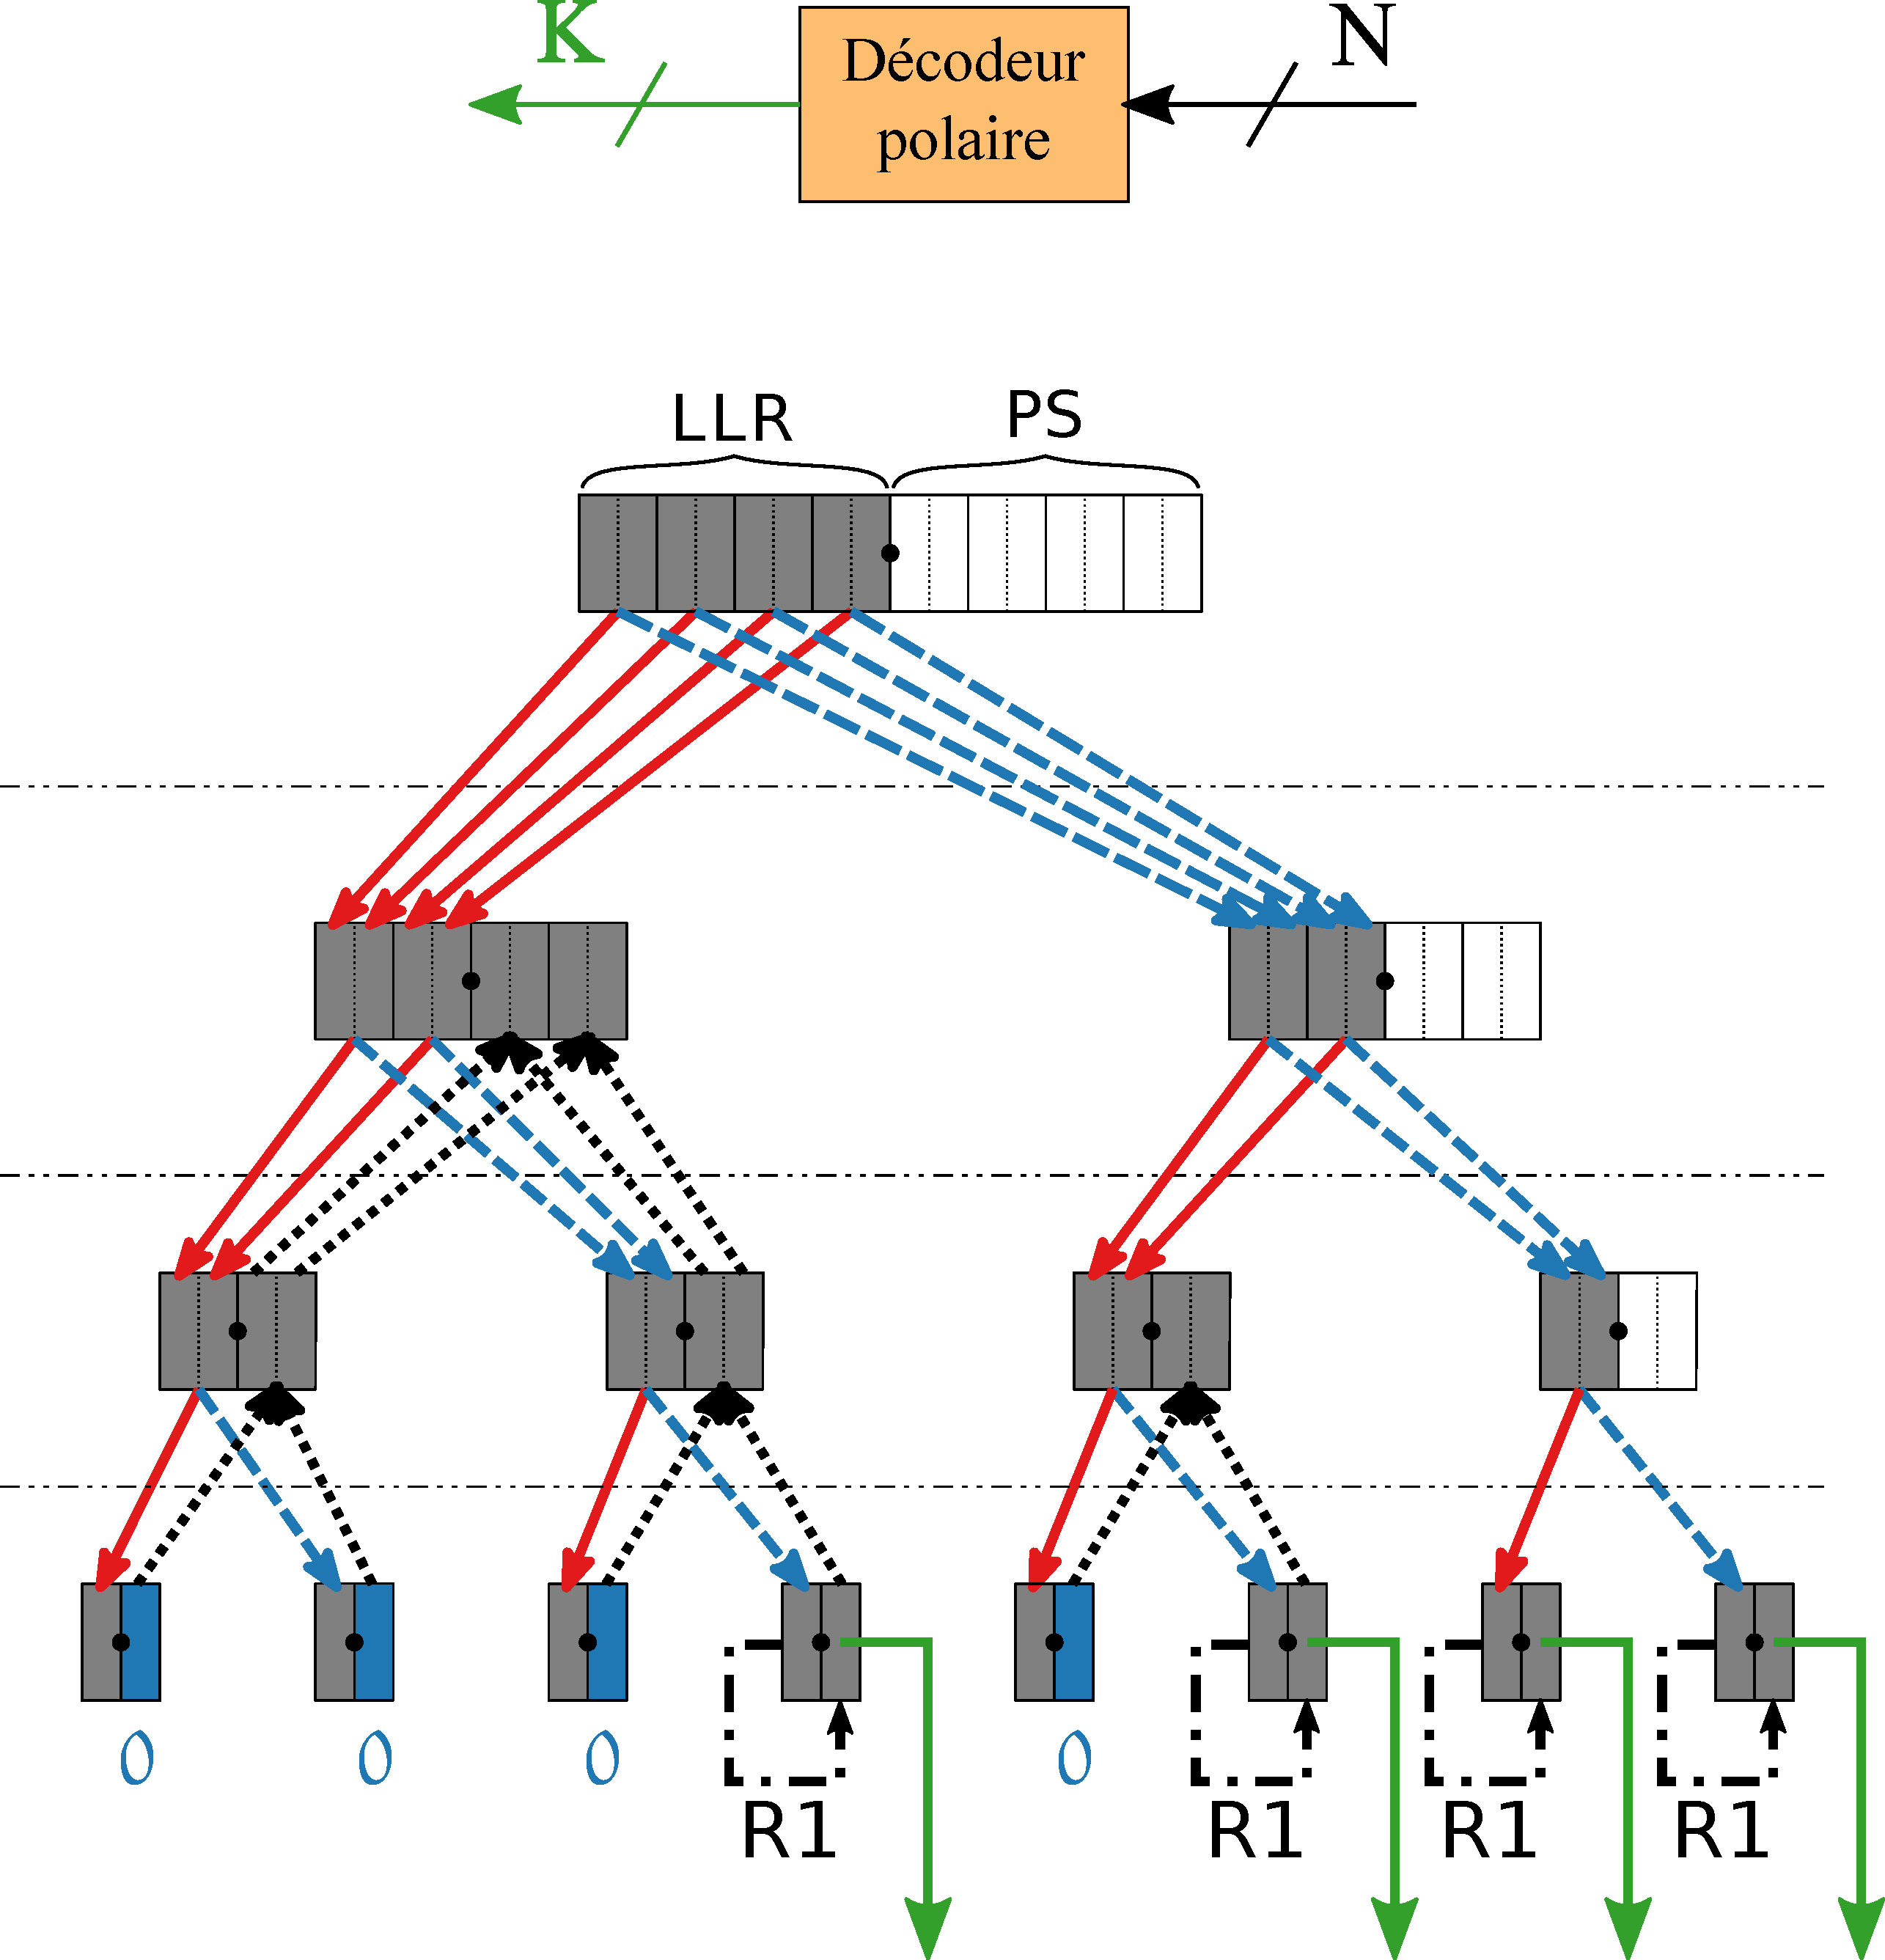
\includegraphics[width=.5\textwidth]{fig/sc_tree_output.pdf}
\end{frame}

\subsection*{Le décodage SC Liste}

\begin{frame}[c]{Algorithme de décodage SCL}
	\begin{columns}[T] % align columns

		\begin{column}{.7\textwidth}

			\multiinclude[<+>][start=1,format=pdf,graphics={width=\textwidth}]{./fig/scl_anim}

		\end{column}

		\begin{column}{.3\textwidth}
			\begin{itemize}
				\item<3-> Pas de décision dure
				\item<4-> Duplication des chemins
				\item<5-> Métrique de chemins
				\item<6-> Tri des métrique \& élimination
				\item<7-> Mot de code décodé
			\end{itemize}
		\end{column}

	\end{columns}
\end{frame}

\begin{frame}[c]{Algorithme de décodage CASCL}
			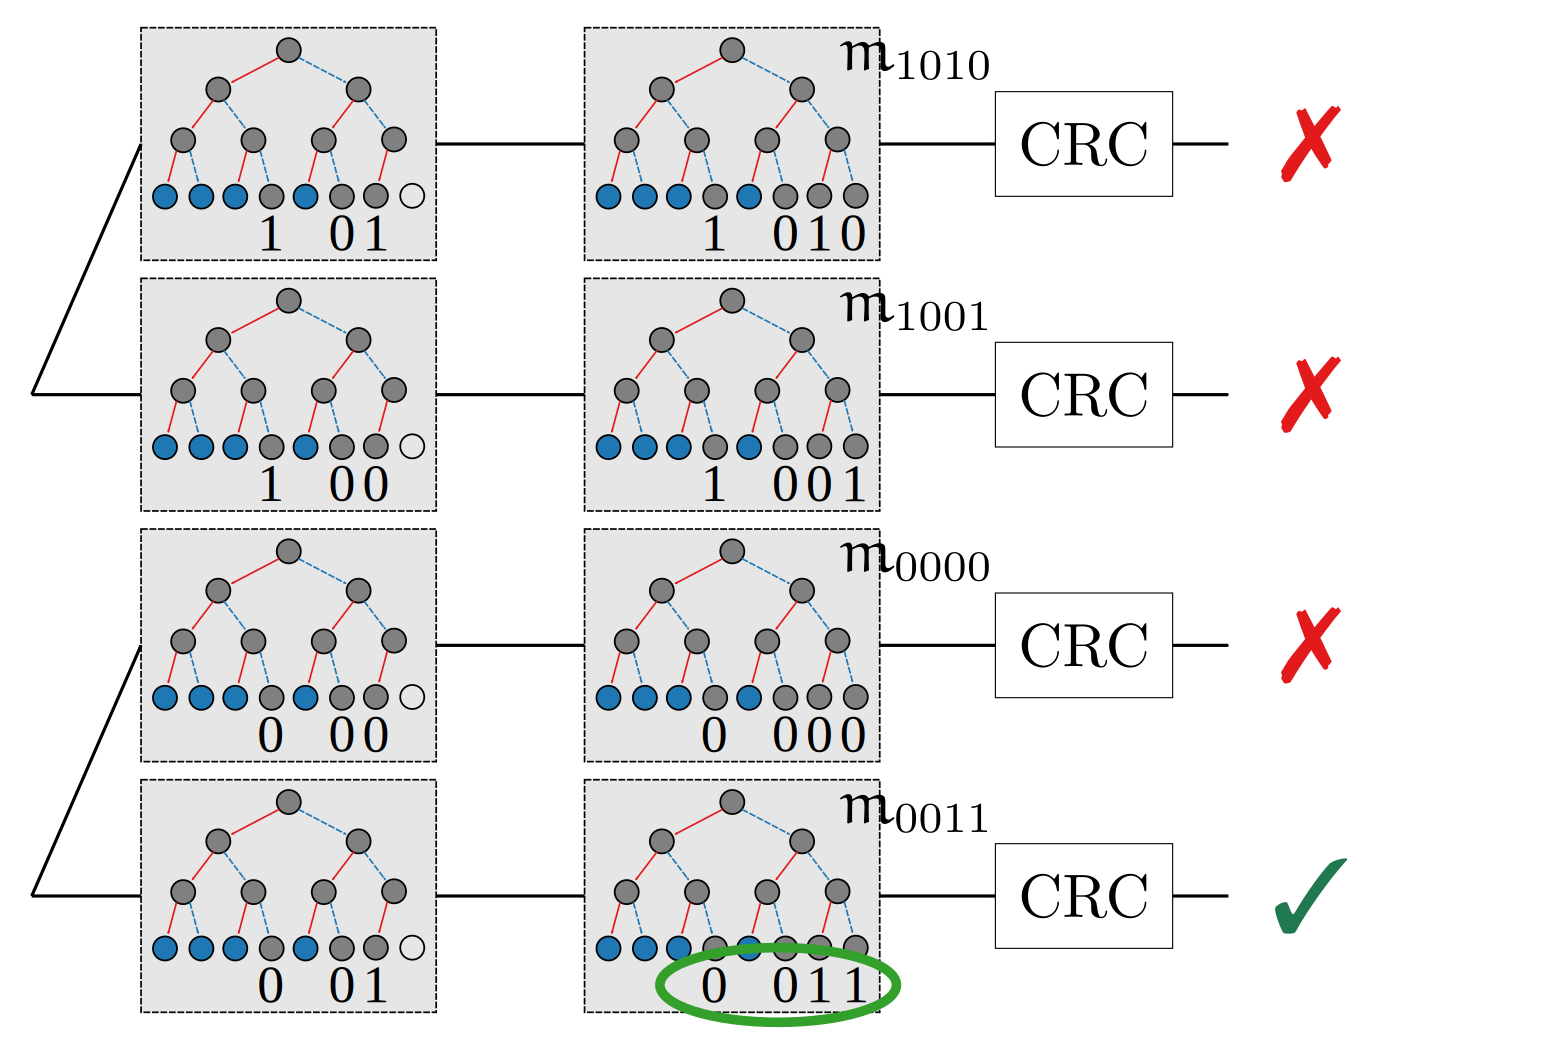
\includegraphics[width=\textwidth]{./fig/cascl}
			\begin{itemize}
				\item Distance faible des codes polaires
				\item Améliorée par la concaténation du CRC
				\item Utilisé pour discriminer les candidats
			\end{itemize}
\end{frame}

\begin{frame}[c]{Performances de décodage}
			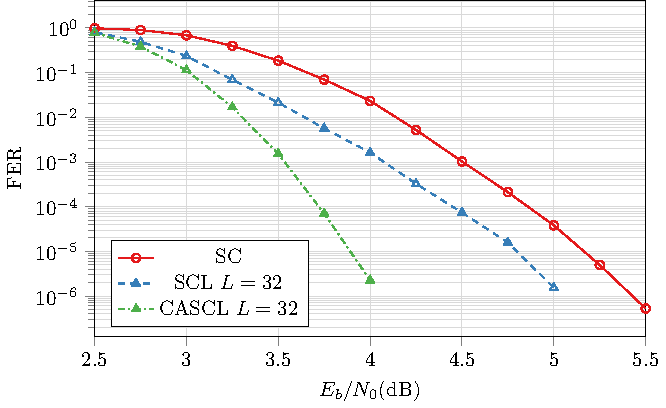
\includegraphics[width=\textwidth]{./fig/scl_L/tikz/source}
\end{frame}

\begin{frame}[c]{\'Elagage de l'arbre}
			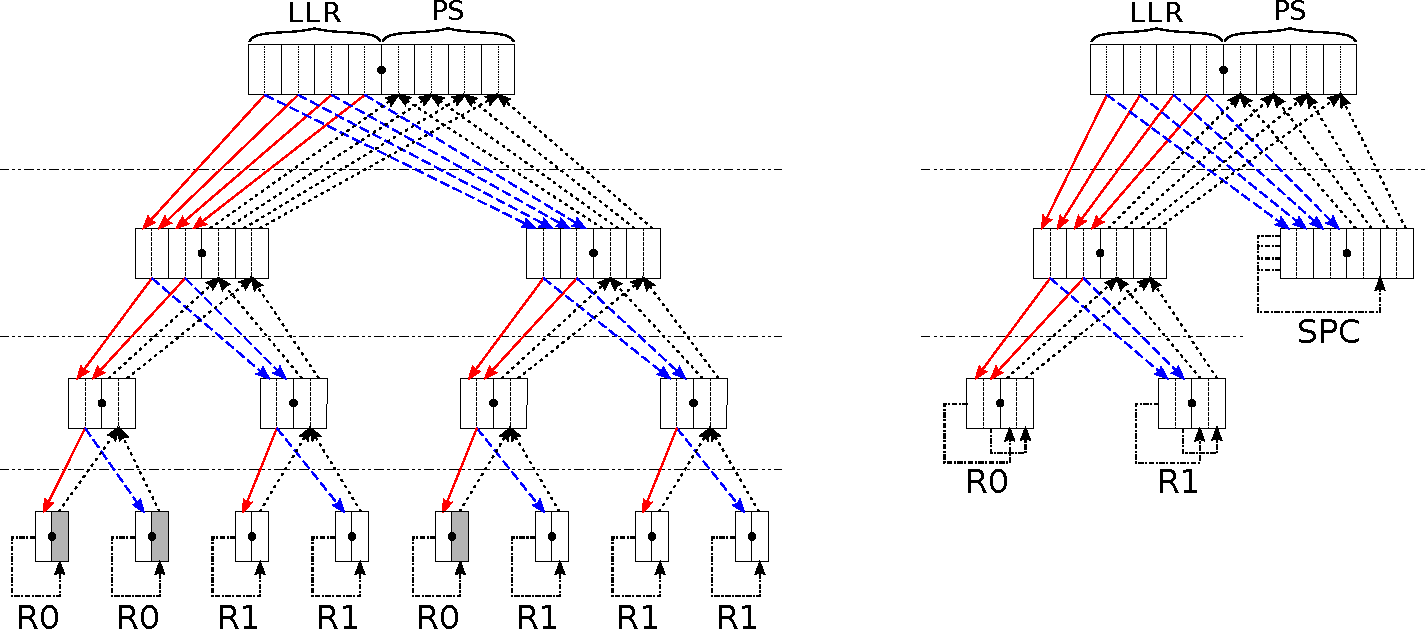
\includegraphics[width=\textwidth]{./fig/pruning}
\end{frame}

\begin{frame}[c]{Algorithmes de décodage}
  \begin{table}[t]
    \centering
    {\small\resizebox{0.8\linewidth}{!}{
     \begin{tabular}{r|c|c|c} 
      \textbf{Algorithme}  & \textbf{Performances}  & \multirow{2}{*}{\textbf{Débit}} & \textbf{Latence}  \\
      \textbf{de décodage} & \textbf{BER \& FER}    &                                 & \textbf{Maximum}  \\
      \hline
      SC           & \RED{faibles}                  & \GREEN{haut}                    & \GREEN{faible}    \\
      SCL          & \ORANGE{moyennes}              & \RED{bas}                       & \ORANGE{moyenne}  \\
      CASCL       & \GREEN{élevées}            & \RED{bas}                       & \ORANGE{moyenne}  \\
      Adaptive-SCL & \GREEN{élevées}            & \GREEN{haut}                    & \RED{forte}       \\
    \end{tabular}
    }}
  \end{table}
	\vspace{0.5cm}
\end{frame}

\begin{frame}[c]{Résumé}
	\begin{itemize}
		\item Chaîne de communications
		\item Role des codes correcteurs d'erreurs
		\item Codes polaires
		\item Algorithme de décodage SC
		\item Algorithme de décodage SCL (et CASCL)
		\item Compromis entre performances de décodage, débit et latence
	\end{itemize}
\end{frame}
\section[Décodeur logiciel à liste]{Décodage à liste sur processeurs génériques}
\subsection*{}

\begin{frame}[c]{\'Evolutions des systèmes de télécommunications}
	\multiinclude[<+>][start=1,format=pdf,graphics={width=\textwidth}]{./fig/bs_evo}
	\begin{itemize}
		\item<1-> Architectures dédiées localisées pour le calcul bande de base
		\item<2-> Architectures dédiées à distance pour le calcul bande de base
		\item<3-> Cloud-RAN : décodeur logiciel
		\item<4-> Adaptativité de l'infrastructure
	\end{itemize}
\end{frame}

\begin{frame}[c]{Décodeur logiciel}
	\begin{itemize}
		\item Algorithmes de décodage dans des langages de haut niveau
		\item Cible : x86 et ARM
		\item Exploitation des unités SIMD
	\end{itemize}
\end{frame}

\begin{frame}[c]{Généricité et Flexibilité}
	\begin{itemize}
		\item Généricité
		\begin{itemize}
			\item N, K
			\item Concaténation de CRC
			\item Position des bits gelés
			\item Poinçonnage
		\end{itemize}
		\item Flexibilité
		\begin{itemize}
			\item Variantes algorithmiques
			\item Taille de la liste
			\item Représentation en virgule fixe
			\item Ajustement de l'élagage
			\item Non déroulé
		\end{itemize}
	\end{itemize}
\end{frame}


\begin{frame}[c]{Généricité et Flexibilité}
  \begin{table}[t]
    \centering
    {\small\resizebox{0.8\linewidth}{!}{
     	\begin{tabular}{r|cccc} 
     	 Décodeur     & \cite{shen_low-latency_2016} & \cite{sarkis_increasing_2014} & \cite{sarkis_fast_2016} & Ce travail  \\
     	\cmidrule(lr){1-1}
     	\cmidrule(lr){2-2}
     	\cmidrule(lr){3-3}
     	\cmidrule(lr){4-4}
     	\cmidrule(lr){5-5}
     	 Code déroulé & \GREEN{NON}                  & \GREEN{NON}                   & \RED{OUI}               & \GREEN{NON} \\
     	 PASCL        & \xmark                       & \cmark                        & \cmark                  & \cmark \\
     	 FASCL        & \xmark                       & \xmark                        & \xmark                  & \cmark \\
     	 Virgule fixe & \xmark                       & \xmark                        & \xmark                  & \cmark \\
     	 \multirow{2}{*}{\'Elagage}    & \multirow{2}{*}{Fixe}                         &  \multirow{2}{*}{Fixe}                           &  \multirow{2}{*}{Fixe}                     & Ajustable \\
     	 & &  &  & Dynamique \\
     	 Poinçonnage & \xmark                       & \xmark                        & \xmark                  & \cmark \\

    	\end{tabular}
    }}
  \end{table}
\end{frame}



\begin{frame}[c]{Impact de l'élagage des nœuds SPC}
	\centering
	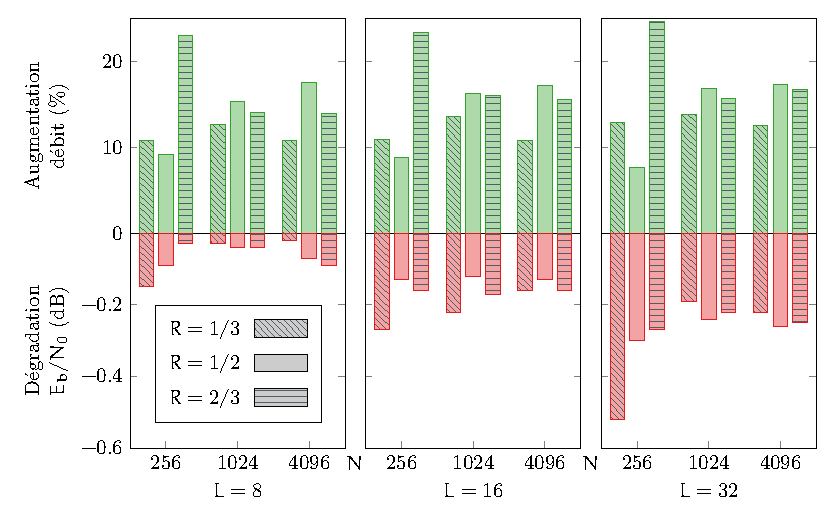
\includegraphics[width=0.7\textwidth]{./fig/thr_spc/tikz/thr_spc_diff}
\end{frame}

\begin{frame}[c]{Représentation en virgule fixe}
  \begin{table}[hb]
    \renewcommand{\arraystretch}{1.1}
    \centering
    {\small\resizebox{\linewidth}{!}{
    \begin{tabular}{r | c | c || c | c || c | c || c | c}
      \multirow{2}{*}{\textbf{Décodeur}} & \multirow{2}{*}{\textbf{Quantif.}} & \multirow{2}{*}{${\mathcal{L}_{PC}}$} & \multicolumn{2}{c ||}{\textbf{3.5 dB}} & \multicolumn{2}{c ||}{\textbf{4.0 dB}} & \multicolumn{2}{c}{\textbf{4.5 dB}} \\
      \cline{4-9}
      & & & ${\mathcal{L}_{moy}}$ & ${\mathcal{T}_i}$ & ${\mathcal{L}_{moy}}$ & ${\mathcal{T}_i}$ & ${\mathcal{L}_{moy}}$ & ${\mathcal{T}_i}$ \\
      % \hline
      \hline
      \multirow{3}{*}{PA-SSCL} & 32-bit &  635 & 232.3 &   7.6 & 41.7 &  42.1 & 7.4 & 237.6 \\
      %\cline{3-9}
                               & 16-bit &  622 & 219.6 &   8.0 & 40.1 &  43.8 & 6.6 & 267.5 \\
      %\cline{3-9}
                               &  8-bit &  651 & 232.4 &   7.6 & 41.2 &  42.6 & 6.5 & 268.3 \\
      \hline
      \multirow{3}{*}{FA-SSCL} & 32-bit & 1201 &  67.2 &  26.1 &  8.5 & 207.8 & 5.1 & 345.5 \\
      %\cline{3-9}
                               & 16-bit & 1198 &  68.7 &  25.6 &  7.7 & 225.7 & 4.3 & 408.7 \\
      %\cline{3-9}
                               &  8-bit & 1259 &  71.8 &  24.4 &  7.7 & 227.3 & 4.1 & 425.9 \\
    \end{tabular}
    }}
   \end{table}
    \begin{itemize}
    	\item Prototypage
    	\item Augmentation du parallélisme
    	\item Augmentation du débit
    \end{itemize}
\end{frame}


\begin{frame}[c]{Déroulage}
\begin{itemize}
	\item Déroulage : génération de code source
	\item Désavantage : manque de flexibilité
	\item Non utilisé dans notre implémentation
	\item Techniques permettant d'augmenter le débit
	\begin{itemize}
		\item Nouvelle technique de tri
		\item Gestion du stockage des sommes partielles
		\item Extraction du CRC
	\end{itemize}
\end{itemize}
\end{frame}


\begin{frame}[c]{Déroulage}
\begin{itemize}
	\item Déroulage : génération de code source
	\item Désavantage : manque de flexibilité
	\item Non utilisé dans notre implémentation
	\item Techniques permettant d'augmenter le débit
	\begin{itemize}
		\item Nouvelle technique de tri
		\item Gestion du stockage des sommes partielles
		\item \textbf{Extraction du CRC}
	\end{itemize}
\end{itemize}
\end{frame}

\begin{frame}[c]{Déroulage}
	\centering
	\multiinclude[<+>][start=1,format=pdf,graphics={width=.7\textwidth}]{./fig/extract}
\end{frame}



\begin{frame}
    \begin{table}[ht]
      \centering
      {\small\resizebox{0.8\linewidth}{!}{
      \begin{tabular}{r|l|c|c|c c c}
        \multirow{2}{*}{\textbf{Cible}} & \multirow{2}{*}{\textbf{Algorithme}} & \multirow{2}{*}{\textbf{Version}}  & \multirow{1}{*}{\textbf{${\mathcal{L}_{PC}}$}} & \multicolumn{3}{c}{${\mathcal{T}_i}$ (Mb/s)} \\
        \cline{5-7}
        &                        &   & ($\mu s$)                          & \textbf{3.5 dB} & \textbf{4.0 dB} & \textbf{4.5 dB} \\
        \hline
        
        i7-4790K & CASCL  &~\cite{shen_low-latency_2016}      & 1572                           & 1.10            & 1.10            & 1.10            \\
        \hline
        i7-2600  & CASCL\textsuperscript{1} &~\cite{sarkis_increasing_2014}     & 23000                          & 0.07            & 0.07            & 0.07            \\
        i7-2600  & CASCL\textsuperscript{1} &~\cite{sarkis_fast_2016}           & 2294                           & 0.76            & 0.76            & 0.76            \\
        i7-2600  & CASCL\textsuperscript{1} & Ce travail                        & 4819                           & 0.37            & 0.37            & 0.37            \\
        i5-6600K & CASCL\textsuperscript{1} & Ce travail                        & 3635                           & 0.48            & 0.48            & 0.48            \\
        \hline
        i7-2600  & CASCL &~\cite{sarkis_increasing_2014}    & 3300                           & 0.52            & 0.52            & 0.52            \\
        i7-2600  & CASCL &~\cite{sarkis_fast_2016}          & 433                            & 4.0             & 4.0             & 4.0             \\
        i7-2600  & CASCL & Ce travail                       & 770                            & 2.3             & 2.3             & 2.3             \\
        i5-6600K & CASCL & Ce travail                       & 577                            & 3.0             & 3.0             & 3.0             \\
        \hline
        i7-2600  & PASCL &~\cite{sarkis_increasing_2014}    & $\approx$ 3300                 & 0.9             & 4.90            & 54.0            \\
        i7-2600  & PASCL &~\cite{sarkis_fast_2016}          & $\approx$ 433                  & 8.6             & 33.0            & 196.0           \\
        i7-2600  & PASCL & Ce travail                       & 847                            & 5.5             & 31.1            & 168.4           \\
        i5-6600K & PASCL & Ce travail                       & 635                            & 7.6             & 42.1            & 237.6           \\
        \hline
        i7-2600  & FASCL & Ce travail                       & 1602                           & 19.4            & 149.0           & 244.3           \\
        i5-6600K & FASCL & Ce travail                       & 1201                           & 26.1            & 207.8           & 345.5           \\
      \end{tabular}
      }}
 
  \end{table}
\end{frame}

\section{Conception d'architectures programmables}



\subsection*{Conception d'architectures programmables}





\begin{frame}[c]{Algorithmes de décodage}
  \begin{table}[t]
    \centering
    {\small\resizebox{0.8\linewidth}{!}{
     \begin{tabular}{r|c|c|c} 
      \textbf{Algorithme}  & \textbf{Performances}  & \multirow{2}{*}{\textbf{Débit}} & \textbf{Latence}  \\
      \textbf{de décodage} & \textbf{BER \& FER}    &                                 & \textbf{Maximum}  \\
      \hline
      SC           & \RED{faibles}                  & \GREEN{haut}                    & \GREEN{faible}    \\
      SCL          & \ORANGE{moyennes}              & \RED{bas}                       & \ORANGE{moyenne}  \\
      CA-SCL       & \GREEN{importantes}            & \RED{bas}                       & \ORANGE{moyenne}  \\
      Adaptive-SCL & \GREEN{importantes}            & \GREEN{haut}                    & \RED{forte}       \\
    \end{tabular}
    }}
  \end{table}
	\vspace{0.5cm}
	\centering
  Tous ces algorithmes sont basés sur l'algorithme SC
  \vspace{0.7cm}

  L'architecture proposée se concentre sur l'algorithme SC
\end{frame}

\centering


\begin{frame}[c]{Des implémentations materielles et logicielles efficaces}

	\begin{minipage}[c][0cm][t]{\textwidth}
	\centering
	\only<1>{Implémentations matérielles dédiées}
	\only<2>{Implémentations logicielles sur des processeurs génériques}
	\only<3>{Tailles de codes et rendements variés}
	\only<4>{Latence en faveur des architectures dédiées}
	\only<5>{Débits compétitifs des décodeurs logiciels}
	\only<6>{Principal défaut des décodeurs logiciels : la consommation énergétique}
	\only<7>{\GREEN{Comment conserver la flexibilité des décodeurs logiciels en se rapprochant des performances des architectures dédiées ?}}
	\end{minipage}		

	\vspace{1cm}
	% \only<+>{
	% \begin{tabular}{ccccccc}
	% \vspace{0.55cm}
	% & & & & & & \\
	% & & & & & & \\
	% & & & & & & \\
	% & & & & & & \\
	% & & & & & & \\
	% & & & & & & \\
	% & & & & & & \\
	% & & & & & & \\
	% % Work           & Platform   &  N                     & R                    & Lat. ($\mu s$)& Thr.(Mb/s) & $E_b$ (nJ/bit)  \\\hline
	% % \cite{6804939} & Stratix IV &  32768                 & 0.9                  & 26.4          & 1200       & -               \\
	% % \cite{8017407} & ASIC 28nm  &  1024                  & 0.5                  & 5.46          & 94         & 0.095           \\
	% % \cite{8017407} & ASIC 28nm  &  1024\footnotemark[1]  & 0.5\footnotemark[1]  & 1.17          & 436        & 0.006           \\\hline
	% % \cite{Giard15} & i7-4770S   &  32768                 & 0.84                 & 31            & 886        & 73              \\
	% % \cite{6960078} & i7-4960HQ  &  32768                 & 0.83                 & 337           & 1400       & 34              \\
	% % \cite{7760327} & Cortex A57 &  32768                 & 0.83                 & 374           & 73         & 27              \\
	% % \cite{Giard15} & Tesla K20c &  4096                  & 0.90                 & 9400          & 1043       & 216             \\
	% \end{tabular}
	% }
	\only<+>{
	\begin{tabular}{c|c|c|c|c|c|c}
	Ref.           & \textbf{Circuit} &  N                     & R                    & Lat. ($\mu s$)& Débit(Mb/s) & $E_b$ (nJ/bit)  \\\hline
	\cite{6804939} & \textbf{Stratix IV} &  32768                 & 0.9                  & 26.4          & 1200       & -               \\
	\cite{7105452} & \textbf{Stratix IV} &  1024\footnotemark[1]  & 0.5\footnotemark[1]  & 2.4           & 237000     & -               \\
	\cite{8017407} & \textbf{ASIC 28nm } &  1024                  & 0.5                  & 5.46          & 94         & 0.095           \\
	\cite{8017407} & \textbf{ASIC 28nm } &  1024\footnotemark[1]  & 0.5\footnotemark[1]  & 1.17          & 436        & 0.006           \\\hline
	\cite{Giard15} & i7-4770S   &  32768                 & 0.84                 & 31            & 886        & 73                       \\
	\cite{6960078} & i7-4960HQ  &  32768                 & 0.83                 & 337           & 1400       & 34                       \\
	\cite{7760327} & Cortex A57 &  32768                 & 0.83                 & 374           & 73         & 27                       \\
	\cite{Giard15} & Tesla K20c &  4096                  & 0.90                 & 9400          & 1043       & 216                      \\
	\end{tabular}
	\footnotetext[1]{\tiny Fixed N \& R}
	}
	\only<+>{
	\begin{tabular}{c|c|c|c|c|c|c}
	Ref.           & \textbf{Circuit  } &  N                     & R                    & Lat. ($\mu s$)& Débit(Mb/s) & $E_b$ (nJ/bit)  \\\hline
	\cite{6804939} & Stratix IV &  32768                 & 0.9                  & 26.4          & 1200       & -                        \\
	\cite{7105452} & Stratix IV &  1024\footnotemark[1]  & 0.5\footnotemark[1]  & 2.4           & 237000     & -                        \\
	\cite{8017407} & ASIC 28nm  &  1024                  & 0.5                  & 5.46          & 94         & 0.095                    \\
	\cite{8017407} & ASIC 28nm  &  1024\footnotemark[1]  & 0.5\footnotemark[1]  & 1.17          & 436        & 0.006                    \\\hline
	\cite{Giard15} & \textbf{i7-4770S  } &  32768                 & 0.84                 & 31            & 886        & 73              \\
	\cite{6960078} & \textbf{i7-4960HQ } &  32768                 & 0.83                 & 337           & 1400       & 34              \\
	\cite{7760327} & \textbf{Cortex A57} &  32768                 & 0.83                 & 374           & 73         & 27              \\
	\cite{Giard15} & \textbf{Tesla K20c} &  4096                  & 0.90                 & 9400          & 1043       & 216             \\
	\end{tabular}
	\footnotetext[1]{\tiny Fixed N \& R}
	}
	\only<+>{
	\begin{tabular}{c|c|c|c|c|c|c}
	Ref.           & Circuit   &  \textbf{N                  }   & \textbf{R                  }  & Lat. ($\mu s$)& Débit(Mb/s) & $E_b$ (nJ/bit)  \\\hline
	\cite{6804939} & Stratix IV &  \textbf{32768              }   & \textbf{0.9                }  & 26.4          & 1200       & -               \\
	\cite{7105452} & Stratix IV &  \textbf{1024\footnotemark[1]}  & \textbf{0.5\footnotemark[1]}  & 2.4           & 237000     & -               \\
	\cite{8017407} & ASIC 28nm  &  \textbf{1024               }   & \textbf{0.5                }  & 5.46          & 94         & 0.095           \\
	\cite{8017407} & ASIC 28nm  &  \textbf{1024\footnotemark[1]}  & \textbf{0.5\footnotemark[1]}  & 1.17          & 436        & 0.006           \\\hline
	\cite{Giard15} & i7-4770S   &  \textbf{32768              }   & \textbf{0.84               }  & 31            & 886        & 73              \\
	\cite{6960078} & i7-4960HQ  &  \textbf{32768              }   & \textbf{0.83               }  & 337           & 1400       & 34              \\
	\cite{7760327} & Cortex A57 &  \textbf{32768              }   & \textbf{0.83               }  & 374           & 73         & 27              \\
	\cite{Giard15} & Tesla K20c &  \textbf{4096               }   & \textbf{0.90               }  & 9400          & 1043       & 216             \\
	\end{tabular}
	\footnotetext[1]{\tiny Fixed N \& R}
	}
		\only<+>{
	\begin{tabular}{c|c|c|c|c|c|c}
	Ref.           & Circuit   &  N                     & R                    & \textbf{Lat.} ($\mathbold{\mu s}$)& Débit(Mb/s) & $E_b$ (nJ/bit)    \\\hline
	\cite{6804939} & Stratix IV &  32768                 & 0.9                  & \GREEN{26.4}                   & 1200       & -         \\
	\cite{7105452} & Stratix IV &  1024\footnotemark[1]  & 0.5\footnotemark[1]  & \GREEN{2.4}                    & 237000     & -               \\
	\cite{8017407} & ASIC 28nm  &  1024                  & 0.5                  & \GREEN{5.46}                   & 94         & 0.095     \\
	\cite{8017407} & ASIC 28nm  &  1024\footnotemark[1]  & 0.5\footnotemark[1]  & \GREEN{1.17}                   & 436        & 0.006     \\\hline
	\cite{Giard15} & i7-4770S   &  32768                 & 0.84                 & \GREEN{31  }                   & 886        & 73        \\
	\cite{6960078} & i7-4960HQ  &  32768                 & 0.83                 & \ORANGE{337}                   & 1400       & 34        \\
	\cite{7760327} & Cortex A57 &  32768                 & 0.83                 & \ORANGE{374}                   & 73         & 27        \\
	\cite{Giard15} & Tesla K20c &  4096                  & 0.90                 & \RED{9400}                     & 1043       & 216       \\
	\end{tabular}
	\footnotetext[1]{\tiny Fixed N \& R}
	}
	\only<+>{
	\begin{tabular}{c|c|c|c|c|c|c}
	Ref.           & Circuit   &  N                     & R                    & Lat. ($\mu s$)& \textbf{Débit(Mb/s)} & $E_b$ (nJ/bit)    \\\hline
	\cite{6804939} & Stratix IV &  32768                 & 0.9                  & 26.4          & \GREEN{1200}       & -                  \\
	\cite{7105452} & Stratix IV &  1024\footnotemark[1]  & 0.5\footnotemark[1]  & 2.4           & \BLUE{237000}      & -                  \\
	\cite{8017407} & ASIC 28nm  &  1024                  & 0.5                  & 5.46          & \ORANGE{94}        & 0.095              \\
	\cite{8017407} & ASIC 28nm  &  1024\footnotemark[1]  & 0.5\footnotemark[1]  & 1.17          & \GREEN{436}        & 0.006              \\\hline
	\cite{Giard15} & i7-4770S   &  32768                 & 0.84                 & 31            & \GREEN{886}        & 73                 \\
	\cite{6960078} & i7-4960HQ  &  32768                 & 0.83                 & 337           & \GREEN{1400}       & 34                 \\
	\cite{7760327} & Cortex A57 &  32768                 & 0.83                 & 374           & \ORANGE{73}        & 27                 \\
	\cite{Giard15} & Tesla K20c &  4096                  & 0.90                 & 9400          & \GREEN{1043}       & 216                \\
	\end{tabular}
	\footnotetext[1]{\tiny Fixed N \& R}
	}
	\only<+>{
	\begin{tabular}{c|c|c|c|c|c|c}
	Ref.           & Circuit   &  N                     & R                    & Lat. ($\mu s$)& Débit(Mb/s) & $\mathbf{E_b}$ \textbf{(nJ/bit)}  \\\hline
	\cite{6804939} & Stratix IV &  32768                 & 0.9                  & 26.4          & 1200       & \textbf{-}                        \\
	\cite{7105452} & Stratix IV &  1024\footnotemark[1]  & 0.5\footnotemark[1]  & 2.4           & 237000     & \textbf{-}                        \\
	\cite{8017407} & ASIC 28nm  &  1024                  & 0.5                  & 5.46          & 94         & \GREEN{0.095}                     \\
	\cite{8017407} & ASIC 28nm  &  1024\footnotemark[1]  & 0.5\footnotemark[1]  & 1.17          & 436        & \GREEN{0.006}                     \\\hline
	\cite{Giard15} & i7-4770S   &  32768                 & 0.84                 & 31            & 886        & \ORANGE{73}                       \\
	\cite{6960078} & i7-4960HQ  &  32768                 & 0.83                 & 337           & 1400       & \ORANGE{34}                       \\
	\cite{7760327} & Cortex A57 &  32768                 & 0.83                 & 374           & 73         & \ORANGE{27}                       \\
	\cite{Giard15} & Tesla K20c &  4096                  & 0.90                 & 9400          & 1043       & \RED{216}                         \\
	\end{tabular}
	\footnotetext[1]{\tiny Fixed N \& R}
	}

	\only<+>{
	\vspace{0.5cm}
	\begin{tabular}{c|c|c|c|c|c|c}
	Ref.           & Circuit   &  N                     & R                    & Lat. ($\mu s$)& Débit(Mb/s) & $E_b$ (nJ/bit)  \\\hline
	\cite{6804939} & Stratix IV &  32768                 & 0.9                  & 26.4          & 1200       & -                        \\
	\cite{7105452} & Stratix IV &  1024\footnotemark[1]  & 0.5\footnotemark[1]  & 2.4           & 237000     & -                        \\
	\cite{8017407} & ASIC 28nm  &  1024                  & 0.5                  & 5.46          & 94         & 0.095                     \\
	\cite{8017407} & ASIC 28nm  &  1024\footnotemark[1]  & 0.5\footnotemark[1]  & 1.17          & 436        & 0.006                     \\\hline
	& \GREEN{?} & \GREEN{?} & \GREEN{?} & \GREEN{?} & \GREEN{?} & \GREEN{?} \\\hline
	\cite{Giard15} & i7-4770S   &  32768                 & 0.84                 & 31            & 886        & 73                       \\
	\cite{6960078} & i7-4960HQ  &  32768                 & 0.83                 & 337           & 1400       & 34                       \\
	\cite{7760327} & Cortex A57 &  32768                 & 0.83                 & 374           & 73         & 27                       \\
	\cite{Giard15} & Tesla K20c &  4096                  & 0.90                 & 9400          & 1043       & 216                         \\
	\end{tabular}
	}

\end{frame}


% \begin{frame}[c]{Goal of this research}
% 	To propose a polar decoder architecture that
% 	\vspace*{1.5cm}
% 	\begin{itemize}
% 		\item<+-> Maintains the genericity of software programmable processors
% 		\item<+-> Increases the throughput
% 		\item<+-> Decreases the energy consumption
% 		\item<+-> May be easily improved to support various algorithms (SCAN, SCF...)
% 	\end{itemize}
% \end{frame}


\begin{frame}[c]{Deux modèles de conception d'ASIP}
	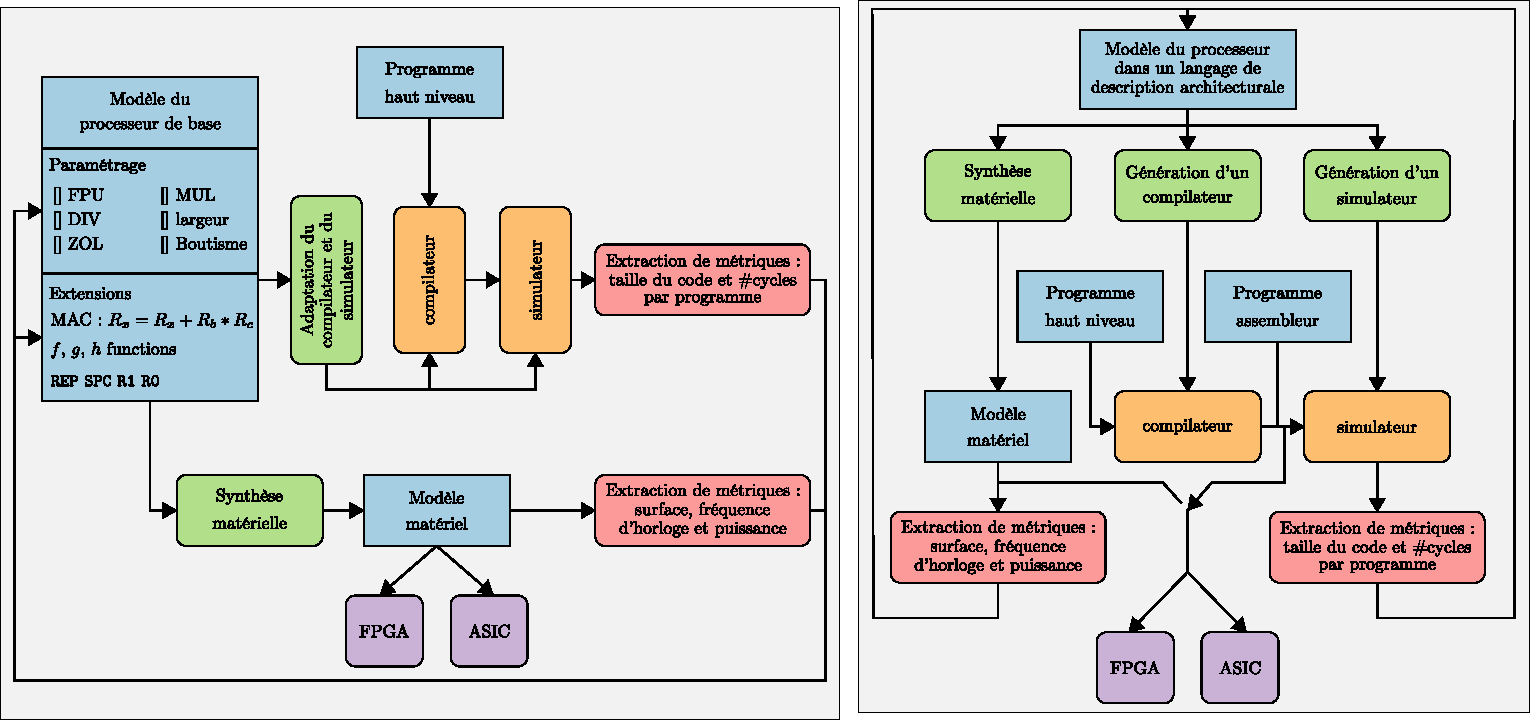
\includegraphics[width=0.9\textwidth]{./fig/methodos}
\end{frame}


\begin{frame}[c]{Limites de l'approche Tensilica}
	\begin{itemize}
		\item Langage de description matérielle spécifique
		\item Licence
		\item Limitation de l'accès à la mémoire
		\item Rigidité de l'architecture
	\end{itemize}
\end{frame}

\begin{frame}[c]{Transport Triggered Architectures}
	\begin{itemize}
		\item Modèle de processeur
		\vspace{0.5cm}
		\item Similaire aux architectures VLIW
		\vspace{0.5cm}
		\item Parallélisme de données
		\vspace{0.5cm}
		\item Parallélisme d'instructions
	\end{itemize}
\end{frame}

\begin{frame}[c]{Structure d'un processeur TTA}
	\multiinclude[<+>][start=1,format=pdf,graphics={width=.8\textwidth}]{./fig/anim_tta_base}
\end{frame}

\begin{frame}[c]{Niveau de parallélisme}
	Two main polar functions : $f$ and $g$
	\vspace{1cm}

	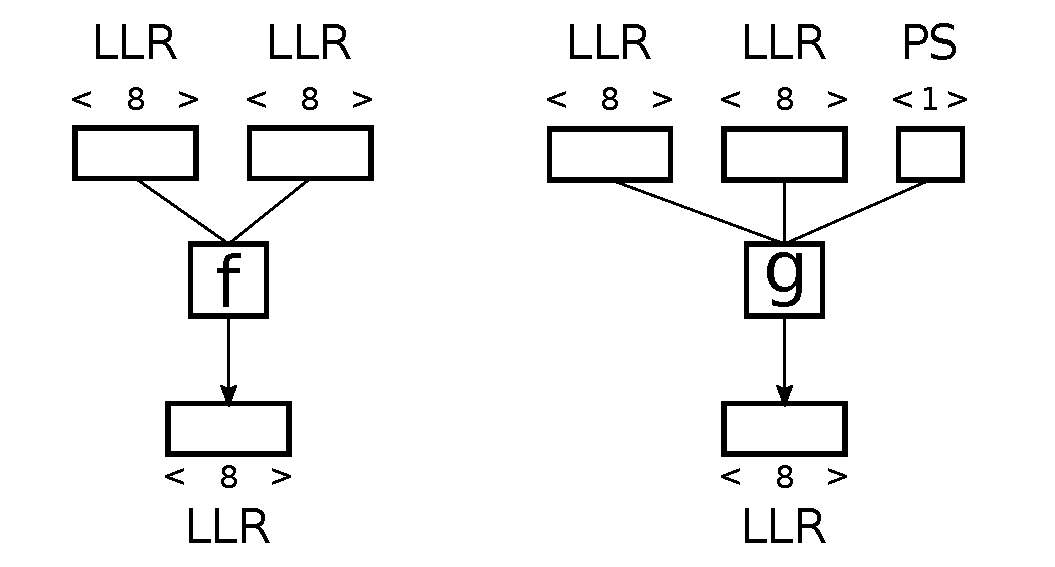
\includegraphics[width=0.7\textwidth]{fig/f_g_dimensions_scalar}
\end{frame}

\begin{frame}[c]{Niveau de parallélisme}
	Two main polar functions : $f$ and $g$
	\vspace{1cm}

	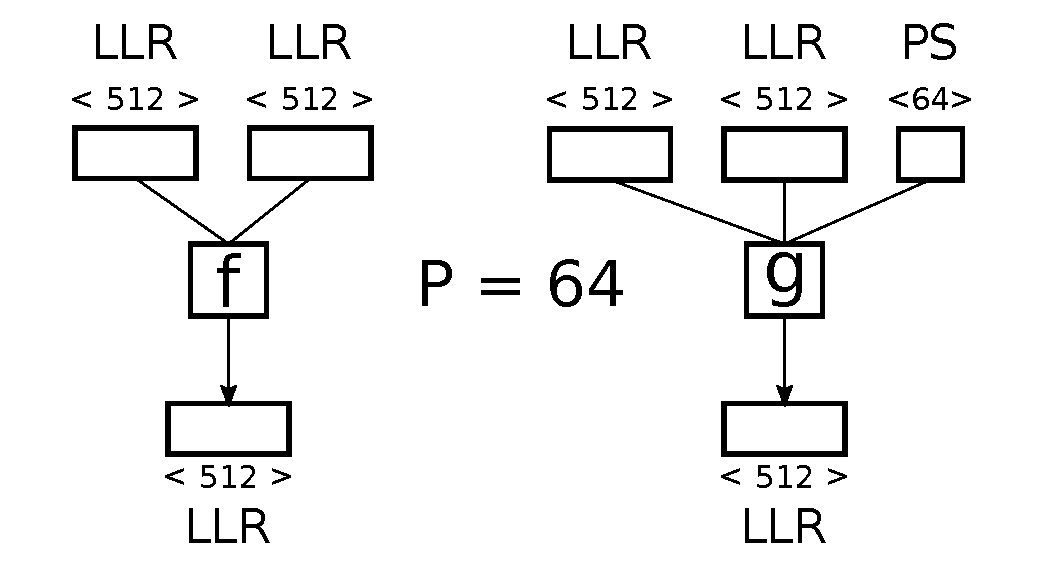
\includegraphics[width=0.7\textwidth]{fig/f_g_dimensions_vector}
\end{frame}

\begin{frame}[c]{Conception du processeur}
	\begin{columns}[T] % align columns
		\begin{column}{.48\textwidth}
			\vspace{-0.5cm}
			\multiinclude[<+>][start=1,format=pdf,graphics={width=1.4\textwidth}]{./fig/archi_sc_construction}
		\end{column}
		\begin{column}{.07\textwidth}
		\end{column}
		\begin{column}{.41\textwidth}
			\begin{itemize}
				\item<1-> Mémoires vectorielles
				\vspace{0.2cm}
				\item<2-> 2 bus de 512 bits
				\vspace{0.2cm}
				\item<2-> 1 bus de 64 bits
				\vspace{0.2cm}
				\item<3-> Unité de chargement et sauvegarde vectorielles
				\vspace{0.2cm}
				\item<4-> Unité de calcul polaire
			\end{itemize}
		\end{column}
	\end{columns} % align columns
\end{frame}

\begin{frame}[c]{Compilation}
	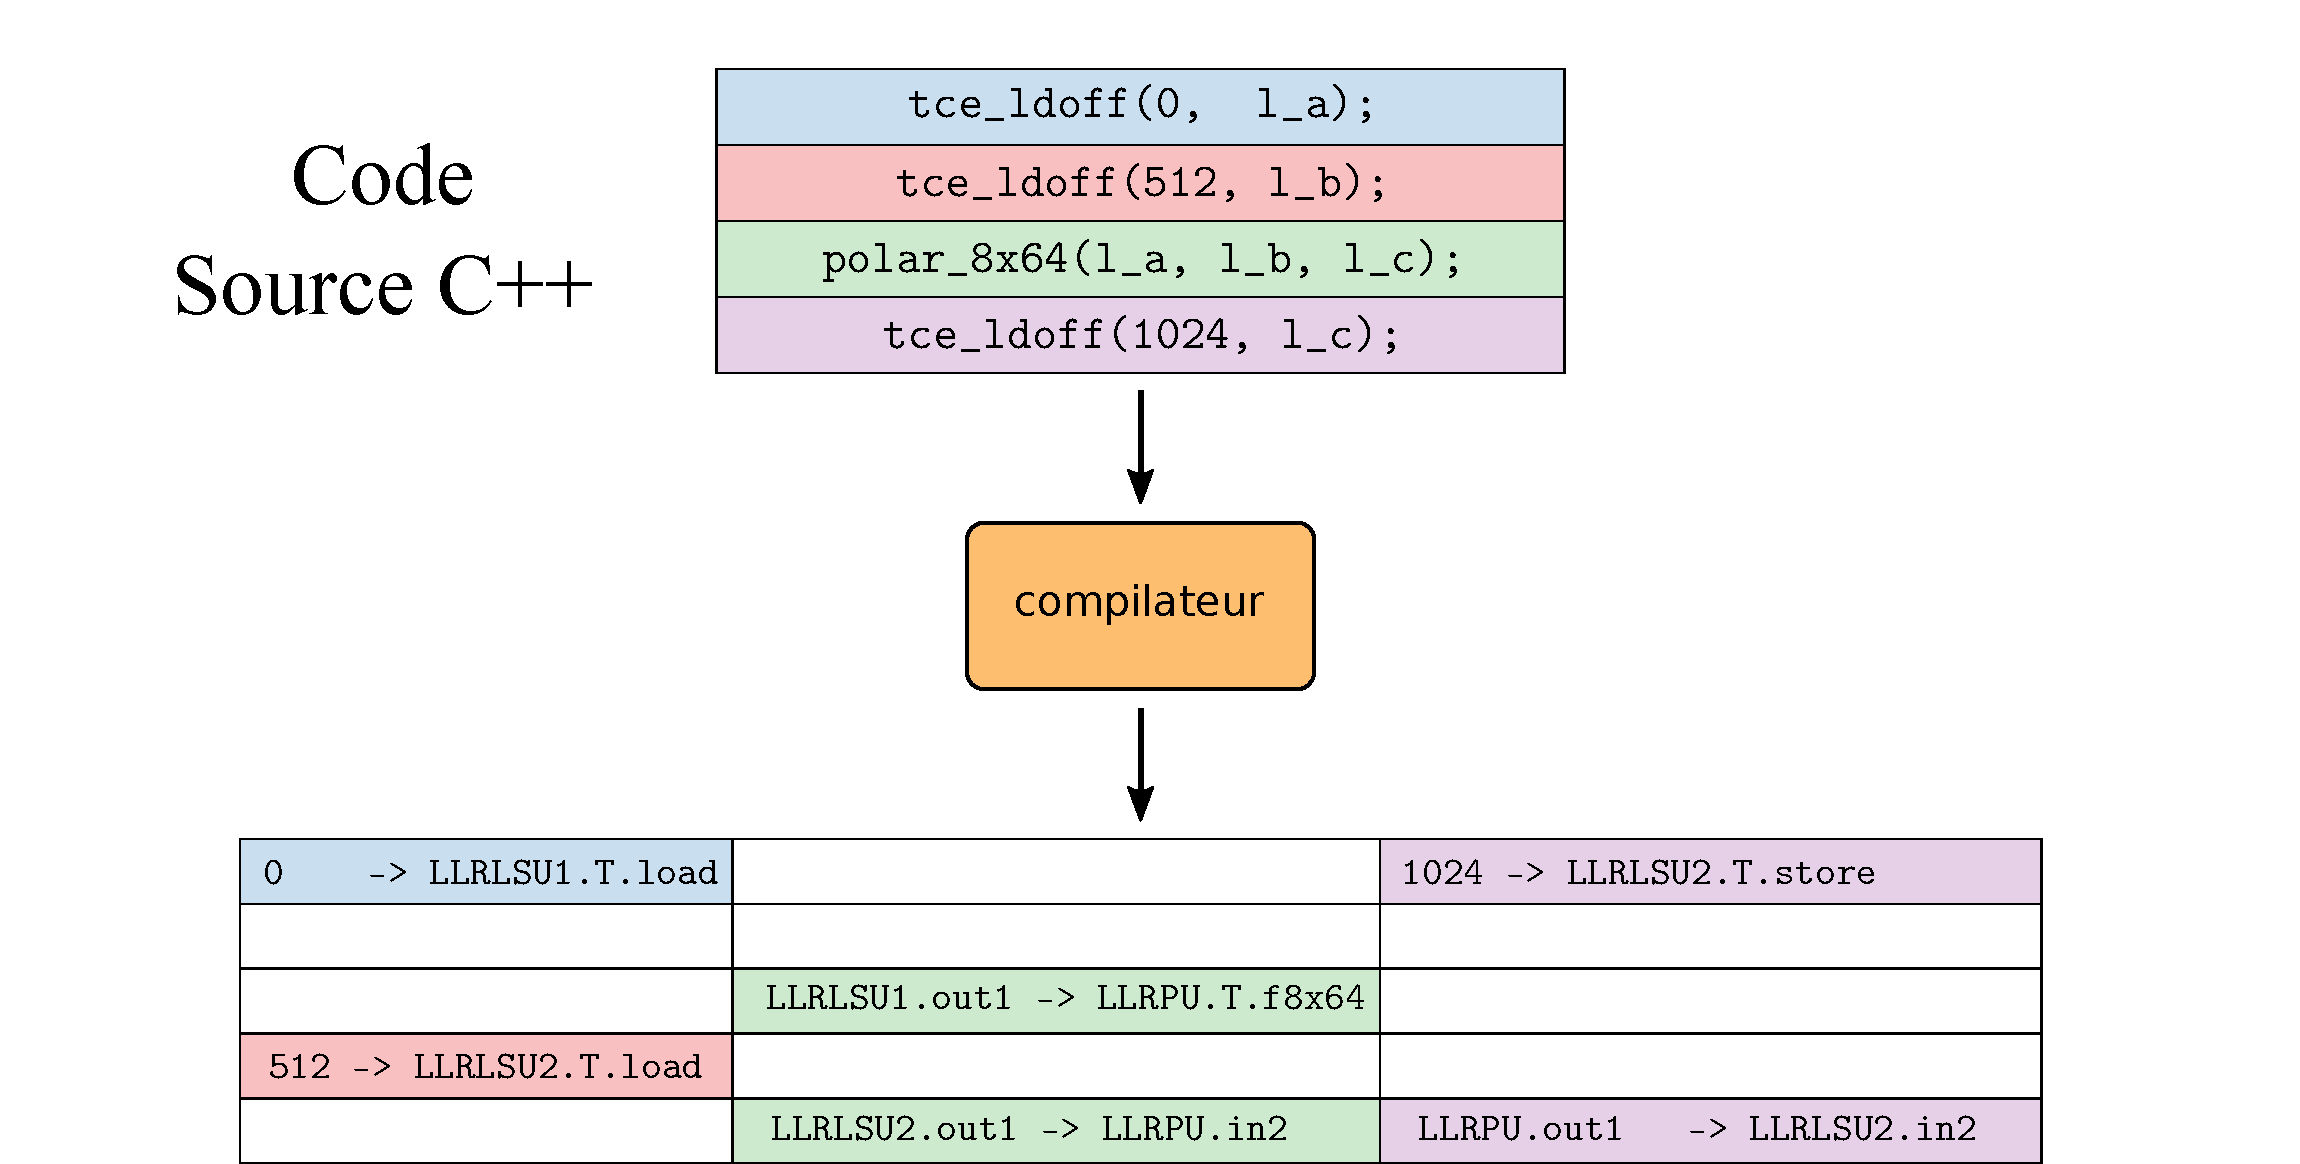
\includegraphics[width=\textwidth]{fig/compilation}
\end{frame}

\begin{frame}[c]{Parallélisme d'instruction}
	\multiinclude[<+>][start=1,format=pdf,graphics={width=.8\textwidth}]{./fig/ilp}
\end{frame}





\begin{frame}[c]{Comparaison avec des décodeurs logiciels}
	\begin{columns}[T] % align columns
	\begin{column}{.48\textwidth}
		\begin{itemize}
			\item<+-> Architecture proposée
			\item<+-> Processeurs Intel x86 (i7-4712HQ) et ARM (Cortex A57)
			\begin{itemize}
				\item<+-> Boîte à outils logicielle \textbf{AFF3CT}
				\item<+-> SIMD (Neon \& AVX2)
			\end{itemize}
			\item<+-> ASIP de type Tensilica
			\item<+-> Débit meximum atteint par le processeur proposé
			\item<+-> Consommation énergétique réduite d'un à deux ordres de grandeur
		\end{itemize}
	\end{column}

	\begin{column}{.48\textwidth}
	\only<1>{
		\begin{table}
			\centering
			{
			\small\resizebox{\linewidth}{!}{
			\begin{tabular}{c|c|c|c|c}
				\toprule

				Architecture & $N$ & \begin{tabular}{c}Latence\\{[$\mu$s]}\end{tabular} & \begin{tabular}{c}Débit\\{[Mb/s]}\end{tabular} & \begin{tabular}{c}$E_b$\\{[nJ/bit]}\end{tabular} \\

				\cmidrule(lr){1-1}
				\cmidrule(lr){2-2}
				\cmidrule(lr){3-5}

				\multirow{2}{*}{\bf \BLUE{TTPD-800MHz}}            & $1024$   & $1.4$  & $352$ & $0.14$ \\ % 1512 cycles
				                                            & $512$    & $0.8$  & $313$ & $0.15$ \\ % 803 cycles
				\multirow{2}{*}{\bf \BLUE{(ASIP)}}                 & $256$    & $0.4$  & $304$ & $0.16$ \\ % 413 cycles
				                                            & $128$    & $0.2$  & $284$ & $0.17$ \\ % 224 cycles
				\midrule
				\multirow{2}{*}{\bf i7-3.3GHz}              & $1024$   & $2.0$  & $257$ & $41$   \\
				                                            & $512$    & $1.2$  & $210$ & $49$   \\
				\multirow{2}{*}{\bf (GPP)}                  & $256$    & $0.7$  & $179$ & $59$   \\
				                                            & $128$    & $0.4$  & $143$ & $73$   \\
				\midrule    
				\multirow{2}{*}{\bf A57-1.1GHz}             & $1024$   & $10.7$ & $48$  & $17$   \\
				                                            & $512$    & $5.3$  & $48$  & $17$   \\
				\multirow{2}{*}{\bf (GPP)}                  & $256$    & $2.8$  & $46$  & $17$   \\
				                                            & $128$    & $1.6$  & $41$  & $20$   \\
				\midrule
				\multirow{2}{*}{\bf LX7-835MHz}             & $1024$   & $7.2$  & $71$  & $1.6$  \\
				                                            & $512$    & $3.9$  & $66$  & $1.7$  \\
				\multirow{2}{*}{\bf (ASIP)}                 & $256$    & $1.9$  & $65$  & $1.7$  \\
				                                            & $128$    & $1.0$  & $62$  & $1.8$  \\
				\bottomrule
			\end{tabular}
			}}
		\end{table}
	}
		
		\only<2-4>{
		\begin{table}
			\centering
			{
			\small\resizebox{\linewidth}{!}{
			\begin{tabular}{c|c|c|c|c}
				\toprule

				Architecture & $N$ & \begin{tabular}{c}Latence\\{[$\mu$s]}\end{tabular} & \begin{tabular}{c}Débit\\{[Mb/s]}\end{tabular} & \begin{tabular}{c}$E_b$\\{[nJ/bit]}\end{tabular} \\

				\cmidrule(lr){1-1}
				\cmidrule(lr){2-2}
				\cmidrule(lr){3-5}


				\multirow{2}{*}{\bf TTPD-800MHz}            & $1024$   & $1.4$  & $352$ & $0.14$ \\ % 1512 cycles
				                                            & $512$    & $0.8$  & $313$ & $0.15$ \\ % 803 cycles
				\multirow{2}{*}{\bf (ASIP)}                 & $256$    & $0.4$  & $304$ & $0.16$ \\ % 413 cycles
				                                            & $128$    & $0.2$  & $284$ & $0.17$ \\ % 224 cycles
				\midrule
				\multirow{2}{*}{\bf \BLUE{i7-3.3GHz}}       & $1024$   & $2.0$  & $257$ & $41$   \\
				                                            & $512$    & $1.2$  & $210$ & $49$   \\
				\multirow{2}{*}{\bf \BLUE{(GPP)}}           & $256$    & $0.7$  & $179$ & $59$   \\
				                                            & $128$    & $0.4$  & $143$ & $73$   \\
				\midrule    
				\multirow{2}{*}{\bf \BLUE{A57-1.1GHz}}      & $1024$   & $10.7$ & $48$  & $17$   \\
				                                            & $512$    & $5.3$  & $48$  & $17$   \\
				\multirow{2}{*}{\bf \BLUE{(GPP)}}           & $256$    & $2.8$  & $46$  & $17$   \\
				                                            & $128$    & $1.6$  & $41$  & $20$   \\
				\midrule
				\multirow{2}{*}{\bf LX7-835MHz}             & $1024$   & $7.2$  & $71$  & $1.6$  \\
				                                            & $512$    & $3.9$  & $66$  & $1.7$  \\
				\multirow{2}{*}{\bf (ASIP)}                 & $256$    & $1.9$  & $65$  & $1.7$  \\
				                                            & $128$    & $1.0$  & $62$  & $1.8$  \\
				\bottomrule
			\end{tabular}
			}}
		\end{table}
		}

	\only<5>{
		\begin{table}
			\centering
			{
			\small\resizebox{\linewidth}{!}{
			\begin{tabular}{c|c|c|c|c}
				\toprule

				Architecture & $N$ & \begin{tabular}{c}Latence\\{[$\mu$s]}\end{tabular} & \begin{tabular}{c}Débit\\{[Mb/s]}\end{tabular} & \begin{tabular}{c}$E_b$\\{[nJ/bit]}\end{tabular} \\

				\cmidrule(lr){1-1}
				\cmidrule(lr){2-2}
				\cmidrule(lr){3-5}


				\multirow{2}{*}{\bf TTPD-800MHz}            & $1024$   & $1.4$  & $352$ & $0.14$ \\ % 1512 cycles
				                                            & $512$    & $0.8$  & $313$ & $0.15$ \\ % 803 cycles
				\multirow{2}{*}{\bf (ASIP)}                 & $256$    & $0.4$  & $304$ & $0.16$ \\ % 413 cycles
				                                            & $128$    & $0.2$  & $284$ & $0.17$ \\ % 224 cycles
				\midrule
				\multirow{2}{*}{\bf i7-3.3GHz}              & $1024$   & $2.0$  & $257$ & $41$   \\
				                                            & $512$    & $1.2$  & $210$ & $49$   \\
				\multirow{2}{*}{\bf (GPP)}                  & $256$    & $0.7$  & $179$ & $59$   \\
				                                            & $128$    & $0.4$  & $143$ & $73$   \\
				\midrule    
				\multirow{2}{*}{\bf A57-1.1GHz}             & $1024$   & $10.7$ & $48$  & $17$   \\
				                                            & $512$    & $5.3$  & $48$  & $17$   \\
				\multirow{2}{*}{\bf (GPP)}                  & $256$    & $2.8$  & $46$  & $17$   \\
				                                            & $128$    & $1.6$  & $41$  & $20$   \\
				\midrule
				\multirow{2}{*}{\bf \BLUE{LX7-835MHz}}      & $1024$   & $7.2$  & $71$  & $1.6$  \\
				                                            & $512$    & $3.9$  & $66$  & $1.7$  \\
				\multirow{2}{*}{\bf \BLUE{(ASIP)}}          & $256$    & $1.9$  & $65$  & $1.7$  \\
				                                            & $128$    & $1.0$  & $62$  & $1.8$  \\

				\bottomrule
			\end{tabular}
			}}
		\end{table}
		}
		\only<6>{
		\begin{table}
			\centering
			{
			\small\resizebox{\linewidth}{!}{
			\begin{tabular}{c|c|c|c|c}
				\toprule

				Architecture & $N$ & \begin{tabular}{c}Latence\\{[$\mu$s]}\end{tabular} & \begin{tabular}{c}Débit\\{[Mb/s]}\end{tabular} & \begin{tabular}{c}$E_b$\\{[nJ/bit]}\end{tabular} \\

				\cmidrule(lr){1-1}
				\cmidrule(lr){2-2}
				\cmidrule(lr){3-5}


				\multirow{2}{*}{\bf TTPD-800MHz}            & $1024$   & $1.4$  & \GREEN{$\mathbf{352}$} & $0.14$ \\ % 1512 cycles
				                                            & $512$    & $0.8$  & \GREEN{$\mathbf{313}$} & $0.15$ \\ % 803 cycles
				\multirow{2}{*}{\bf (ASIP)}                 & $256$    & $0.4$  & \GREEN{$\mathbf{304}$} & $0.16$ \\ % 413 cycles
				                                            & $128$    & $0.2$  & \GREEN{$\mathbf{284}$} & $0.17$ \\ % 224 cycles
				\midrule
				\multirow{2}{*}{\bf i7-3.3GHz}              & $1024$   & $2.0$  & \GREEN{$\mathbf{257}$} & $41$   \\
				                                            & $512$    & $1.2$  & \GREEN{$\mathbf{210}$} & $49$   \\
				\multirow{2}{*}{\bf (GPP)}                  & $256$    & $0.7$  & \GREEN{$\mathbf{179}$} & $59$   \\
				                                            & $128$    & $0.4$  & \GREEN{$\mathbf{143}$} & $73$   \\
				\midrule    
				\multirow{2}{*}{\bf A57-1.1GHz}             & $1024$   & $10.7$ & \ORANGE{$\mathbf{48}$} & $17$   \\
				                                            & $512$    & $5.3$  & \ORANGE{$\mathbf{48}$} & $17$   \\
				\multirow{2}{*}{\bf (GPP)}                  & $256$    & $2.8$  & \ORANGE{$\mathbf{46}$} & $17$   \\
				                                            & $128$    & $1.6$  & \ORANGE{$\mathbf{41}$} & $20$   \\
				\midrule
				\multirow{2}{*}{\bf LX7-835MHz}             & $1024$   & $7.2$  & \ORANGE{$\mathbf{71}$} & $1.6$  \\
				                                            & $512$    & $3.9$  & \ORANGE{$\mathbf{66}$} & $1.7$  \\
				\multirow{2}{*}{\bf (ASIP)}                 & $256$    & $1.9$  & \ORANGE{$\mathbf{65}$} & $1.7$  \\
				                                            & $128$    & $1.0$  & \ORANGE{$\mathbf{62}$} & $1.8$  \\

				\bottomrule
			\end{tabular}
			}}
		\end{table}
		}
		\only<7>{
		\begin{table}
			\centering
			{
			\small\resizebox{\linewidth}{!}{
			\begin{tabular}{c|c|c|c|c}
				\toprule

				Architecture & $N$ & \begin{tabular}{c}Latence\\{[$\mu$s]}\end{tabular} & \begin{tabular}{c}Débit\\{[Mb/s]}\end{tabular} & \begin{tabular}{c}$E_b$\\{[nJ/bit]}\end{tabular} \\

				\cmidrule(lr){1-1}
				\cmidrule(lr){2-2}
				\cmidrule(lr){3-5}


				\multirow{2}{*}{\bf TTPD-800MHz}            & $1024$   & $1.4$  & $352$ & \GREEN{$\mathbf{0.14}$} \\ % 1512 cycles
				                                            & $512$    & $0.8$  & $313$ & \GREEN{$\mathbf{0.15}$} \\ % 803 cycles
				\multirow{2}{*}{\bf (ASIP)}                 & $256$    & $0.4$  & $304$ & \GREEN{$\mathbf{0.16}$} \\ % 413 cycles
				                                            & $128$    & $0.2$  & $284$ & \GREEN{$\mathbf{0.17}$} \\ % 224 cycles
				\midrule
				\multirow{2}{*}{\bf i7-3.3GHz}              & $1024$   & $2.0$  & $257$ & \RED{$\mathbf{41}$}   \\
				                                            & $512$    & $1.2$  & $210$ & \RED{$\mathbf{49}$}   \\
				\multirow{2}{*}{\bf (GPP)}                  & $256$    & $0.7$  & $179$ & \RED{$\mathbf{59}$}   \\
				                                            & $128$    & $0.4$  & $143$ & \RED{$\mathbf{73}$}   \\
				\midrule    
				\multirow{2}{*}{\bf A57-1.1GHz}             & $1024$   & $10.7$ & $48$  & \RED{$\mathbf{17}$}   \\
				                                            & $512$    & $5.3$  & $48$  & \RED{$\mathbf{17}$}   \\
				\multirow{2}{*}{\bf (GPP)}                  & $256$    & $2.8$  & $46$  & \RED{$\mathbf{17}$}   \\
				                                            & $128$    & $1.6$  & $41$  & \RED{$\mathbf{20}$}   \\
				\midrule
				\multirow{2}{*}{\bf LX7-835MHz}             & $1024$   & $7.2$  & $71$  & \ORANGE{$\mathbf{1.6}$}  \\
				                                            & $512$    & $3.9$  & $66$  & \ORANGE{$\mathbf{1.7}$}  \\
				\multirow{2}{*}{\bf (ASIP)}                 & $256$    & $1.9$  & $65$  & \ORANGE{$\mathbf{1.7}$}  \\
				                                            & $128$    & $1.0$  & $62$  & \ORANGE{$\mathbf{1.8}$}  \\

				\bottomrule
			\end{tabular}
			}}
		\end{table}
		}
	\end{column}
	\end{columns}
\end{frame}


\begin{frame}[c]{Comparaison avec des architectures matérielles dédiées}
		\begin{itemize}
			\item<+-> Processeur proposé
			\item<+-> Décodeur matériel dédié
			\item<2-> Décodeur matériel dédié avec construction optimisée
			\item<+-> Implémentations FPGA
		\end{itemize}

		\only<1>{
			\begin{table}
			\centering
			{
				\small\resizebox{0.8\linewidth}{!}{
				\begin{tabular}{c|c|c|c|c}
					                        & \BLUE{TTPD Proposé}  & \cite{giard_638_2015} & \multicolumn{2}{c}{\cite{sarkis2014fast}} \\
					\cmidrule(lr){2-2}
					\cmidrule(lr){3-3}
					\cmidrule(lr){4-5}

					\textbf{FPGA}               &  Artix 7       & Stratix IV            & Stratix IV         & Virtex 6             \\
					\textbf{Cycles d'horloge}   &  1161          & 222                   & 165                & 165                  \\
					\textbf{\'Elagage}          &  R0 \& R1      & Complet               & Complet            & Complet              \\
					\textbf{LUTS}               &  14744         & 23020                 & 24821              & 22115                \\
					\textbf{RAM} (Kb)           &  141           & 43                    & 36                 & 36                   \\

				\end{tabular}
			}}
			\end{table}
		}

		\only<2>{
			\begin{table}
			\centering
			{
				\small\resizebox{0.8\linewidth}{!}{
				\begin{tabular}{c|c|c|c|c}
					                        & TTPD Proposé  & \BLUE{\cite{giard_638_2015}} & \multicolumn{2}{c}{\BLUE{\cite{sarkis2014fast}}} \\
					\cmidrule(lr){2-2}
					\cmidrule(lr){3-3}
					\cmidrule(lr){4-5}

					\textbf{FPGA}         &  Artix 7       & Stratix IV            & Stratix IV         & Virtex 6             \\
					\textbf{Cycles d'horloge}   &  1161          & 222                   & 165                & 165                  \\
					\textbf{\'Elagage}        &  R0 \& R1      & Complet                  & Complet               & Complet                 \\
					\textbf{LUTS}           &  14744         & 23020                 & 24821              & 22115                \\
					\textbf{RAM} (Kb)       &  141           & 43                    & 36                 & 36                   \\

				\end{tabular}
			}}
			\end{table}
		}

		\only<3>{
			\begin{table}
			\centering
			{
				\small\resizebox{0.8\linewidth}{!}{
				\begin{tabular}{c|c|c|c|c}
					                        & TTPD Proposé  & \cite{giard_638_2015} & \multicolumn{2}{c}{\cite{sarkis2014fast}} \\
					\cmidrule(lr){2-2}
					\cmidrule(lr){3-3}
					\cmidrule(lr){4-5}

					\textbf{FPGA}         &  \textbf{Artix 7}       & \textbf{Stratix IV}            & \textbf{Stratix IV }        & \textbf{Virtex 6}             \\
					\textbf{Cycles d'horloge}   &  1161          & 222                   & 165                & 165                  \\
					\textbf{\'Elagage}        &  R0 \& R1      & Complet                  & Complet               & Complet                 \\
					\textbf{LUTS}           &  14744         & 23020                 & 24821              & 22115                \\
					\textbf{RAM} (Kb)       &  141           & 43                    & 36                 & 36                   \\

				\end{tabular}
			}}
			\end{table}
		}
\end{frame}

\begin{frame}[c]{Comparaison avec des architectures matérielles dédiées}
		\begin{itemize}
			\item<+-> 5 à six fois plus de cycles
			\item<+-> Différents niveaux d'élagage
			\item<+-> Plus petit nombre de LUTs
			\item<+-> Plus grosse empreinte mémoire
		\end{itemize}

		\only<1>{
			\begin{table}
			\centering
			{
				\small\resizebox{0.8\linewidth}{!}{
				\begin{tabular}{c|c|c|c|c}
					                        & TTPD Proposé  & \cite{giard_638_2015} & \multicolumn{2}{c}{\cite{sarkis2014fast}} \\
					\cmidrule(lr){2-2}
					\cmidrule(lr){3-3}
					\cmidrule(lr){4-5}

					\textbf{FPGA}         &  Artix 7       & Stratix IV            & Stratix IV         & Virtex 6             \\
					\textbf{Cycles d'horloge}   &  \textbf{1161}  & \textbf{222}           & \textbf{165}        & \textbf{165}          \\
					\textbf{\'Elagage}        &  R0 \& R1      & Complet                  & Complet               & Complet                 \\
					\textbf{LUTS}           &  14744         & 23020                 & 24821              & 22115                \\
					\textbf{RAM} (Kb)       &  141           & 43                    & 36                 & 36                   \\

				\end{tabular}
			}}
			\end{table}
		}
		\only<2>{
			\begin{table}
			\centering
			{
				\small\resizebox{0.8\linewidth}{!}{
				\begin{tabular}{c|c|c|c|c}
					                        & TTPD Proposé  & \cite{giard_638_2015} & \multicolumn{2}{c}{\cite{sarkis2014fast}} \\
					\cmidrule(lr){2-2}
					\cmidrule(lr){3-3}
					\cmidrule(lr){4-5}

					\textbf{FPGA}         &  Artix 7       & Stratix IV            & Stratix IV         & Virtex 6             \\
					\textbf{Cycles d'horloge}   &  1161          & 222                   & 165                & 165                  \\
					\textbf{\'Elagage}        &  \textbf{R0 \& R1}      & \textbf{Complet}                  & \textbf{Complet}               & \textbf{Complet}                 \\
					\textbf{LUTS}           &  14744         & 23020                 & 24821              & 22115                \\
					\textbf{RAM} (Kb)       &  141           & 43                    & 36                 & 36                   \\

				\end{tabular}
			}}
			\end{table}
		}
		\only<3>{
			\begin{table}
			\centering
			{
				\small\resizebox{0.8\linewidth}{!}{
				\begin{tabular}{c|c|c|c|c}
					                        & TTPD Proposé  & \cite{giard_638_2015} & \multicolumn{2}{c}{\cite{sarkis2014fast}} \\
					\cmidrule(lr){2-2}
					\cmidrule(lr){3-3}
					\cmidrule(lr){4-5}

					\textbf{FPGA}         &  Artix 7        & Stratix IV             & Stratix IV          & Virtex 6              \\
					\textbf{Cycles d'horloge}   &  1161           & 222                    & 165                 & 165                   \\
					\textbf{\'Elagage}        &  R0 \& R1       & Complet                   & Complet                & Complet                  \\
					\textbf{LUTS}           &  \textbf{14744} & \textbf{23020}         & \textbf{24821}      & \textbf{22115}        \\
					\textbf{RAM} (Kb)       &  141            & 43                     & 36                  & 36                    \\


				\end{tabular}
			}}
			\end{table}
		}
		\only<4>{
			\begin{table}
			\centering
			{
				\small\resizebox{0.8\linewidth}{!}{
				\begin{tabular}{c|c|c|c|c}
					                        & TTPD Proposé  & \cite{giard_638_2015} & \multicolumn{2}{c}{\cite{sarkis2014fast}} \\
					\cmidrule(lr){2-2}
					\cmidrule(lr){3-3}
					\cmidrule(lr){4-5}

					\textbf{FPGA}         &  Artix 7       & Stratix IV            & Stratix IV         & Virtex 6             \\
					\textbf{Cycles d'horloge}   &  1161          & 222                   & 165                & 165                  \\
					\textbf{\'Elagage}        &  R0 \& R1      & Complet                  & Complet               & Complet                  \\
					\textbf{LUTS}           &  14744         & 23020                 & 24821              & 22115                \\
					\textbf{RAM} (Kb)       &  \textbf{141}  & \textbf{43}           & \textbf{36}        & \textbf{36}          \\


				\end{tabular}
			}}
			\end{table}
		}
\end{frame}

\section{Conclusion et perspectives}
\subsection*{}

\begin{frame}[c]{Conclusion}

	\begin{itemize}
		\item<+-> Premier décodeur polaire TTA
		\vspace{0.3cm}
		\item<+-> Meilleure efficacité énergétique que pour des processeurs embarqués
		\vspace{0.3cm}
		\item<+-> Architecture modulaire et adaptive (implémentation de l'algorithme SCAN)
		\vspace{0.3cm}
		\item<+-> Perspectives
		\begin{itemize}
			\item<+-> Algorithme SCL
			\item<+-> Multicœur
		\end{itemize}
	\end{itemize}

\end{frame}

\begin{frame}[allowframebreaks]{References}
\printbibliography
\end{frame}
\end{document}



% \begin{frame}[c]{Hardware Implementations Comparison}
% 		\begin{table}


% {\small\resizebox{\linewidth}{!}{
% 	\begin{tabular}{c|c|c|c|c|c|c}
% 	Ref.           & Platform    &  N                     & R                    & Lat. ($\mu s$)& Débit(Mb/s) & $E_b$ (nJ/bit)  \\\hline
% 	Ce travail     & ASIP 835MHz &  1024                  & 0.5                  & 7.2           & 71         & 1.6             \\
% 	Ce travail     & ASIP 400MHz &  1024                  & 0.5                  & 15            & 34         & 1.4             \\\hline
% 	\cite{6804939} & Stratix IV  &  32768                 & 0.9                  & 26.4          & 1200       & -               \\
% 	\cite{8017407} & ASIC 28nm   &  1024                  & 0.5                  & 5.46          & 94         & 0.095           \\
% 	\cite{8017407} & ASIC 28nm   &  1024\footnotemark[1]  & 0.5\footnotemark[1]  & 1.17          & 436        & 0.006           \\
% 	\end{tabular}

% }}
% 		\end{table}
% 	\footnotetext[1]{\tiny Fixed N \& R}
% \end{frame}

% \end{document}





% \begin{table}
%   \centering
%   \caption{Comparison of programmable processors running the SC decoding algorithm for R=0.5 polar codes}
%   \label{tab:sw}
% %\scriptsize
%   \begin{tabularx}{.45\textwidth}{ccYYY}
%     \toprule

%     Architecture & $N$ & \begin{tabular}{c}Latence\\{[$\mu$s]}\end{tabular} & \begin{tabular}{c}Débit\\{[Mb/s]}\end{tabular} & \begin{tabular}{c}$E_b$\\{[nJ/bit]}\end{tabular} \\

%     \cmidrule(lr){1-1}
%     \cmidrule(lr){2-2}
%     \cmidrule(lr){3-5}

%     \multirow{2}{*}{\bf i7-3.3GHz}              & $1024$   & $2.0$  & $257$ & $41$ \\
    
%                                                 & $512$    & $1.2$  & $210$ & $49$ \\
    
%     \multirow{2}{*}{\bf (GPP)}                  & $256$    & $0.7$  & $179$ & $59$ \\
    
%                                                 & $128$    & $0.4$  & $143$ & $73$ \\
    
%     \midrule    \multirow{2}{*}{\bf A57-1.1GHz} & $1024$   & $10.7$ & $48$  & $17$ \\

%                                                 & $512$    & $5.3$  & $48$  & $17$ \\

%      \multirow{2}{*}{\bf (GPP)}                 & $256$    & $2.8$  & $46$  & $17$ \\

%                                                 & $128$    & $1.6$  & $41$  & $20$ \\

%     \midrule

%     \multirow{2}{*}{\bf LX7-835MHz}             & $1024$   & $7.2$  & $71$  & $1.6$ \\

%                                                 & $512$    & $3.9$  & $66$  & $1.7$ \\

%      \multirow{2}{*}{\bf (ASIP)}                & $256$    & $1.9$  & $65$  & $1.7$ \\

%                                                 & $128$    & $1.0$  & $62$  & $1.8$ \\

%     \midrule

%     \multirow{2}{*}{\bf TTPD-800MHz}            & $1024$  & $1.4$   & $352$ & $0.14$   \\ % 1512 cycles

%                                                 & $512$    & $0.8$  & $313$ & $0.15$   \\ % 803 cycles

%      \multirow{2}{*}{\bf (ASIP)}                & $256$    & $0.4$  & $304$ & $0.16$   \\ % 413 cycles

%                                                 & $128$    & $0.2$  & $284$ & $0.17$   \\ % 224 cycles

%     \bottomrule
%   \end{tabularx}
% \end{table}


% \begin{table}[ht]
%   %\renewcommand{\arraystretch}{0.5} 
%   %\tabcolsep=6pt
%   \centering
%   \caption{FPGA implementations of dedicated SC decoders for a (1024,512) polar code}
%   \label{tab:fpga}
%   \begin{tabularx}{\linewidth}{rcccc}
%    \toprule

%      & TTPD Proposé  & \cite{giard_638_2015} & \multicolumn{2}{c}{\cite{sarkis2014fast}} \\
% 	\cmidrule(lr){2-2}
% 	\cmidrule(lr){3-3}
% 	\cmidrule(lr){4-5}

%     \textbf{FPGA}         &  Artix 7  & Stratix IV & Stratix IV & Virtex 6 \\
%     \textbf{Clock cycles}   &  1161     & 222        & 165        & 165      \\
%     \textbf{IT/P} (Mb/s)    &  44       & 238        & 319        & 217      \\
%     \textbf{Freq} (MHz)     &  100      & 103        & 103        & 70       \\
%     \textbf{LUTS}           &  14744    & 23020      &  24821     & 22115    \\
%     \textbf{FFs}            &  7354     & 1024       &  5823      & 7941     \\
%     \textbf{RAM} (Kb)       &  141      & 43         &  36        & 36       \\
%     \textbf{\'Elagage}        &  R0 \& R1 & Complet       & Complet       & Complet     \\
%     \bottomrule
%   \end{tabularx}  
% \end{table}
